\documentclass[a4paper,UKenglish]{lipics}
%This is a template for producing LIPIcs articles. 
%See lipics-manual.pdf for further information.
%for A4 paper format use option "a4paper", for US-letter use option "letterpaper"
%for british hyphenation rules use option "UKenglish", for american hyphenation rules use option "USenglish"
% for section-numbered lemmas etc., use "numberwithinsect"
 
\usepackage{lineno}
\linenumbers
\usepackage{microtype}%if unwanted, comment out or use option "draft"

%\graphicspath{{./graphics/}}%helpful if your graphic files are in another directory

% Author macros::begin %%%%%%%%%%%%%%%%%%%%%%%%%%%%%%%%%%%%%%%%%%%%%%%%
\title{A linear-time algorithm for the geodesic center of a simple polygon}
\titlerunning{A linear-time algorithm for the geodesic center of a simple polygon} %optional, in case that the title is too long; the running title should fit into the top page column

\author[1]{Some Authors}
\author[2]{Some more}
\affil[1]{Dummy University Computing Laboratory\\
  Address, Country\\
  \texttt{open@dummyuni.org}}
\affil[2]{Department of Informatics, Dummy College\\
  Address, Country\\
  \texttt{access@dummycollege.org}}
\authorrunning{J.\,Q. Open and J.\,R. Access} %mandatory. First: Use abbreviated first/middle names. Second (only in severe cases): Use first author plus 'et. al.'


\newcommand{\n}[1]{\ensuremath{n_{\scriptscriptstyle M}(#1)}}
\newcommand{\F}[2]{\ensuremath{F_{\scriptscriptstyle #1}(#2)}}
\newcommand{\f}[2]{\ensuremath{f_{\scriptscriptstyle #1}(#2)}}
\newcommand{\fn}[2]{\ensuremath{S_{\scriptscriptstyle #1}(#2)}}
\newcommand{\ff}[1]{\ensuremath{f(#1)}}
\newcommand{\cp}{\ensuremath{c_P}}

\newcommand{\g}[2]{\ensuremath{|\pi(#1, #2)|}}
\newcommand{\p}[2]{\ensuremath{\pi(#1, #2)}}

\newcommand{\SF}[1]{\ensuremath{\mathcal S_{#1}}}

%%
%% Here you may place your macros using \newcommand{}{}
%%


  
  \newcommand{\red}{\color{red}}

\begin{document}

\maketitle

\begin{abstract}
Let $P$ be a simple polygon with $n$ vertices. 
Given two points in $P$, its geodesic distance is the length of the shortest path that connects them among all paths that stay within $P$. The  geodesic center of $P$ is the unique point in $P$ that minimizes the largest geodesic distance to all other points of $P$. In 1989, Pollack, Sharir and Rote [Disc. \& Comput. Geom. 89] showed an $O(n\log n)$-time algorithm to compute the geodesic center of $P$. Since then, a longstanding question, posed also by Mitchell [Handbook of Computational Geometry, 2000],  has been whether this running time can be improved. 
In this paper, we affirmatively answer this question and present a linear time algorithm to solve this problem.
\end{abstract}


%A category including the fourth, optional field follows..

\section{Introduction}
Let $P$ be a simple polygon with $n$ vertices. 
Given two points $x,y\in P$, the \emph{geodesic path} $\p{x}{y}$ is the shortest-path contained in $P$ connecting $x$ with $y$. Notice that if the straight-line segment connecting $x$ with $y$ is contained in $P$, then $\p{x}{y}$ is a straight-line segment. Otherwise, $\p{x}{y}$ is a polygonal chain containing only reflex vertices of $P$ other than its endpoints. (For more information on geodesic paths refer to~\cite{m-gspno-00}).

The \emph{geodesic distance} between $x$ and $y$, denoted by $\g{x}{y}$, is the sum of the Euclidean lengths of each segment in $\p{x}{y}$.
Throughout this paper, when referring to the distance between two points in $P$, we refer to the geodesic distance between them.

The  \emph{geodesic center} of $P$ is the unique point $\cp\in P$ that minimizes the largest geodesic distance to all other points of $P$. 
In 1989, Pollack, Sharir and Rote~\cite{pollackComputingCenter} presented an $O(n\log n)$-time algorithm for computing $\cp$, and since then it has been open whether the running time can be improved. 
In this paper, we affirmatively answer this question by providing an algorithm running in $O(n)$ time. 

The algorithm proposed by Pollack et al.~\cite{pollackComputingCenter} could be summarized as follows: 
Given chord $C$ of $P$ that splits the polygon into two sub-polygons, they describe an algorithm that decides which sub-polygon contains $\cp$. Using this decision algorithm together with the set of chords of a triangulation of $P$, they narrow the search of $P$ to a triangle in which optimization techniques can be used to find $\cp$.
Their approach however, does not allow them to reduce the complexity of the problem on each iteration and hence it runs in $\Theta(n\log n)$ time. We overcome this issue using the following approach.

Given a point $x\in P$, the \emph{farthest neighbor} of $x$, $\ff{x}$, is the point of $P$ that is farthest from $x$. 
Let $\F{P}{x}$ be the function such that for each $x\in P$, $\F{P}{x} = \g{x}{\ff{x}}$.
Note that $\cp$ is the point of $P$ that minimizes the value of  $\F{P}{x}$.

Our algorithms computes a set of $O(n)$ functions of constant description, 
each defined in a triangular domain contained in $P$,
such that their upper envelope, $\phi(x)$, coincides with $\F{P}{x}$.
Thus, we can ``ignore'' the polygon $P$ and focus only on finding the minimum of the function $\phi(x)$.

Because $\phi(x)$ is defined using $O(n)$ functions having triangular domains, 
we are able to use a prune and search approach using cuttings as follows:
We first find a suitable set of $O(n)$ chords of $P$ that splits the polygon into convex regions having constant size.
Our objective is then to find the convex region that contains $\cp$. 
To this end, we use a cuttings of these chords. This cutting has constant complexity and splits $P$ into $O(1)$ cells. 
We then find the cell that contains $\cp$ and recurse on this cell as a new subproblem having smaller complexity. 
To decrease the complexity of the problem, we consider only the functions defined in this cell in the next iteration. 
Using the properties of the cutting, we show that the size of the subproblem decreases by a constant fraction which leads to a linear running time. 
This algorithm has however two stopping conditions, 
one is to reach a subproblem of constant size, 
and a second one is to find a convex trapezoid containing $\cp$.
In the latter case, we are not able to proceed with the prune and search. 
Nevertheless, by restricting the search space to a convex object, 
we show that $\phi(x)$ is a convex function in this domain and hence, 
we are able to use optimization techniques using 
cuttings in $\mathbb{R}^3$ to find the geodesic center in linear time. 

\subsection{Previous Work}
Since the early 80s the problem of computing the geodesic center (and its counterpart, the geodesic diameter) has received a lot of attention from the computational geometry community. Chazelle~\cite{c-tpca-82} gave the first algorithm for computing the geodesic diameter (which ran in $O(n^2)$ time using linear space). Afterwards, Suri~\cite{suri1989computing} reduced it to $O(n\log n)$-time without increasing the space constraints. Finally, Hershberger and Suri~\cite{hershberger1993matrix} presented a fast matrix search technique one of whose applications was a linear-time algorithm for computing the diameter.

The first algorithm for computing the geodesic center was given by Asano and Toussaint~\cite{at-cgcsp-85}, and runs in $O(n^4\log n)$-time. Later Pollack, Sharir, and Rote~\cite{pollackComputingCenter} improved it to $O(n\log n)$ time. Since then, it has been a open problem whether the geodesic center can be
computed in linear time (indeed, this problem was explicitly posed by Mitchell~\cite{m-gspno-00}).

Several other variations of these two problems have been considered. Nowadays there exist algorithms for computing the center and diameter under different metrics. Namely, the $L_1$ geodesic distance~\cite{bkow-clgdcsplt-13},  the link distance~\cite{suri-mlpprp-87,k-ealdp-89,dls-aclcsp-92} (where we look for the path with the minimum possible number of bends or {\em links}), or even rectilinear link distance~\cite{ns-crldp-91,ns-oarlcrp-96} (a variation of the link distance in which only isothetic segments are allowed). The diameter and center of a simple polygon for both the $L_1$ and rectilinear link metrics can be computed in linear time (whereas $O(n\log n)$ time is needed for the link distance).

Another natural extension is the computation of the diameter and center in polygonal domains (i.e., polygons with one or more holes). Polynomial time algorithms are known for both the diameter~\cite{bko-gdpd-13} and center~\cite{bko-cgcpd-14}, although the running times are significantly larger (i.e., $O(n^{7.73})$ and $O(n^{12+\varepsilon})$, respectively).

\subsection{Outline}
To guide the reader, we provide a rough sketch of our algorithm.
As mentioned above, the main idea of the algorithm is to compute a set of triangles whose union covers $P$ such that:
(1) each triangle has a distance function defined in it and (2) the upper envelope $\phi(x)$ has a minimum that coincides with $\F{P}{x}$.

More formally, for each point $x\in P$, there is one triangle containing $x$ and a function $g$ defined in this triangle, such that $g(x) = \F{P}{x}$. Intuitively, we compute a set of functions that ``shatter'' $\F{P}{x}$ into small pieces. 
To compute these triangles and their corresponding functions, we proceed as follows.

In Section~\ref{Section:Decomposing the boundary}, we use the matrix search technique introduced by Hershberger and Suri~\cite{hershberger1993matrix} to compute the farthest neighbor of each vertex of $P$. 
In this way, we partition the boundary of $P$, denoted by $\partial P$, into connected edge disjoint chains,
each grouping the vertices of $P$ that share the same farthest neighbor. 
We say that a vertex is \emph{marked} if it is represented by a chain in this partition of the boundary (not all vertices are marked). 
Further, this partition induces \emph{transition edges} whose endpoints have different farthest neighbors. 

In Section~\ref{Section: Building hourglasses}, we consider each transition edge $ab$ of $\partial P$ independently and compute its \emph{hourglass}. The hourglass $H_{ab}$ of $ab$ is the geodesic convex hull of $a,b, \ff{a}$ and $\ff{b}$, recall that $\ff{a}$ and $\ff{b}$ denote the farthest neighbors of $a$ and $b$, respectively . 
We show that the sum of the complexities of each hourglass defined on a transition edge is $O(n)$. 
Moreover, we show how to compute these hourglasses in linear time.

In Section~\ref{Section:Computing apexed triangles} we show how to compute the triangles and their respective functions.
We distinguish two cases: (1) Inside each hourglass $H_{ab}$ of a transition edge, we use the shortest-path trees of $a$ and $b$ in $H_{ab}$ to decompose $H_{ab}$ into $O(|H_{ab}|)$ triangles with their respective functions. 
(2) For each marked vertex $v$ we compute triangles that encode the distance from $v$. Moreover, we guarantee that these triangles cover every point of $P$ whose farthest neighbor is $v$. Overall, we compute $O(n)$ triangles and we show that this can be done in $O(n)$ time.

As mentioned before, once our set of triangles (and their respective set of functions) is computed, in Section~\ref{section:Prune and search} we use cuttings to narrow the search for $\cp$ to a constant size convex domain.
Because $\phi(x)$ is a convex function when restricted to this domain, in Section~\ref{Section:Solving convex optimization poblem} we show how to use cuttings in $\mathbb{R}^3$ to find the point that minimizes the value of $\phi(x)$. Both steps again run in $O(n)$ time, which leads to an overall linear running time of the algorithm to compute the geodesic center of $P$.



\section{Preliminaries}
Given a point $x\in P$, let $\f{P}{x}$ (or simply $\ff{x}$ when the context is clear) denote the vertex of $P$ that is (geodesically) farthest from $x$ (if two or more vertices are at the same distance from $x$, we choose one of them arbitrarily). 


Let $\F{P}{x} = \g{x}{\ff{x}}$, i.e., $\F{P}{x}$ is the distance from $x$ to its farthest neighbor in $P$. 
Another way to think of the function $\F{P}{x}$ is as the upper envelope of all the (geodesic) distance functions from $x$ to the vertices of $P$. This is related with the farthest-point geodesic Voronoi diagram of the vertices of $P$. The \emph{Voronoi cell} of a vertex $v$ of $P$ is the set of points $R(v) = \{x\in P : \F{P}{x} = \g{x}{v}\}$ (including boundary points).

In this paper, we represent the function $\F{P}{x}$ using a set of constant complexity distance functions defined on triangles contained in $P$ in such a way that the union of these triangles covers $P$. Moreover, the upper envelope of these functions coincides with $\F{P}{x}$.
Then, we proceed to prune and search for the geodesic center of $P$ by restricting our search to a sub-polygon of $P$ and the triangles that cover this sub-polygon. By pruning a constant fraction of these triangles on each iteration, we are able to obtain a near-linear time algorithm to compute the geodesic center of $P$. The bottleneck of this algorithm comes from computing the set of triangles that covers $P$ and their respective distance functions.


\section{Hourglasses and Funnels}
In this section, we introduce the main tools that are going to be used by the algorithm. Some of the result presented in this section have been shown before in different papers. For most of them, we present proof sketches.

\subsection{Hourglasses}

Given two points $x$ and $y$ on $\partial P$, let $\partial P(x,y)$ be the polygonal chain that starts at $x$ and follows the boundary of $P$ clockwise until reaching $y$.

Let $C = (p_0, p_1, \ldots, p_k)$ be a polygonal chain contained in $\partial P$ sorted in clockwise order.
The \emph{hourglass} of $C$, denoted by $H_C$, is the simple polygon contained in $P$ bounded by $C$, $\p{p_k}{\ff{p_0}}$, $\partial P(\ff{p_0}, \ff{p_k})$ and $\p{\ff{p_k}}{ p_0}$; see Figure~\ref{fig:Transition chains and hourglasses}. 
We call $C$ and $\partial P(\ff{p_0}, \ff{p_k})$ the \emph{top} and \emph{bottom} chains of $H_C$, respectively, while $\p{p_k}{ \ff{p_0}}$ and $\p{\ff{p_k}}{p_0}$ are referred to as the \emph{walls} of $H_C$.

\begin{figure}[tb]
\centering
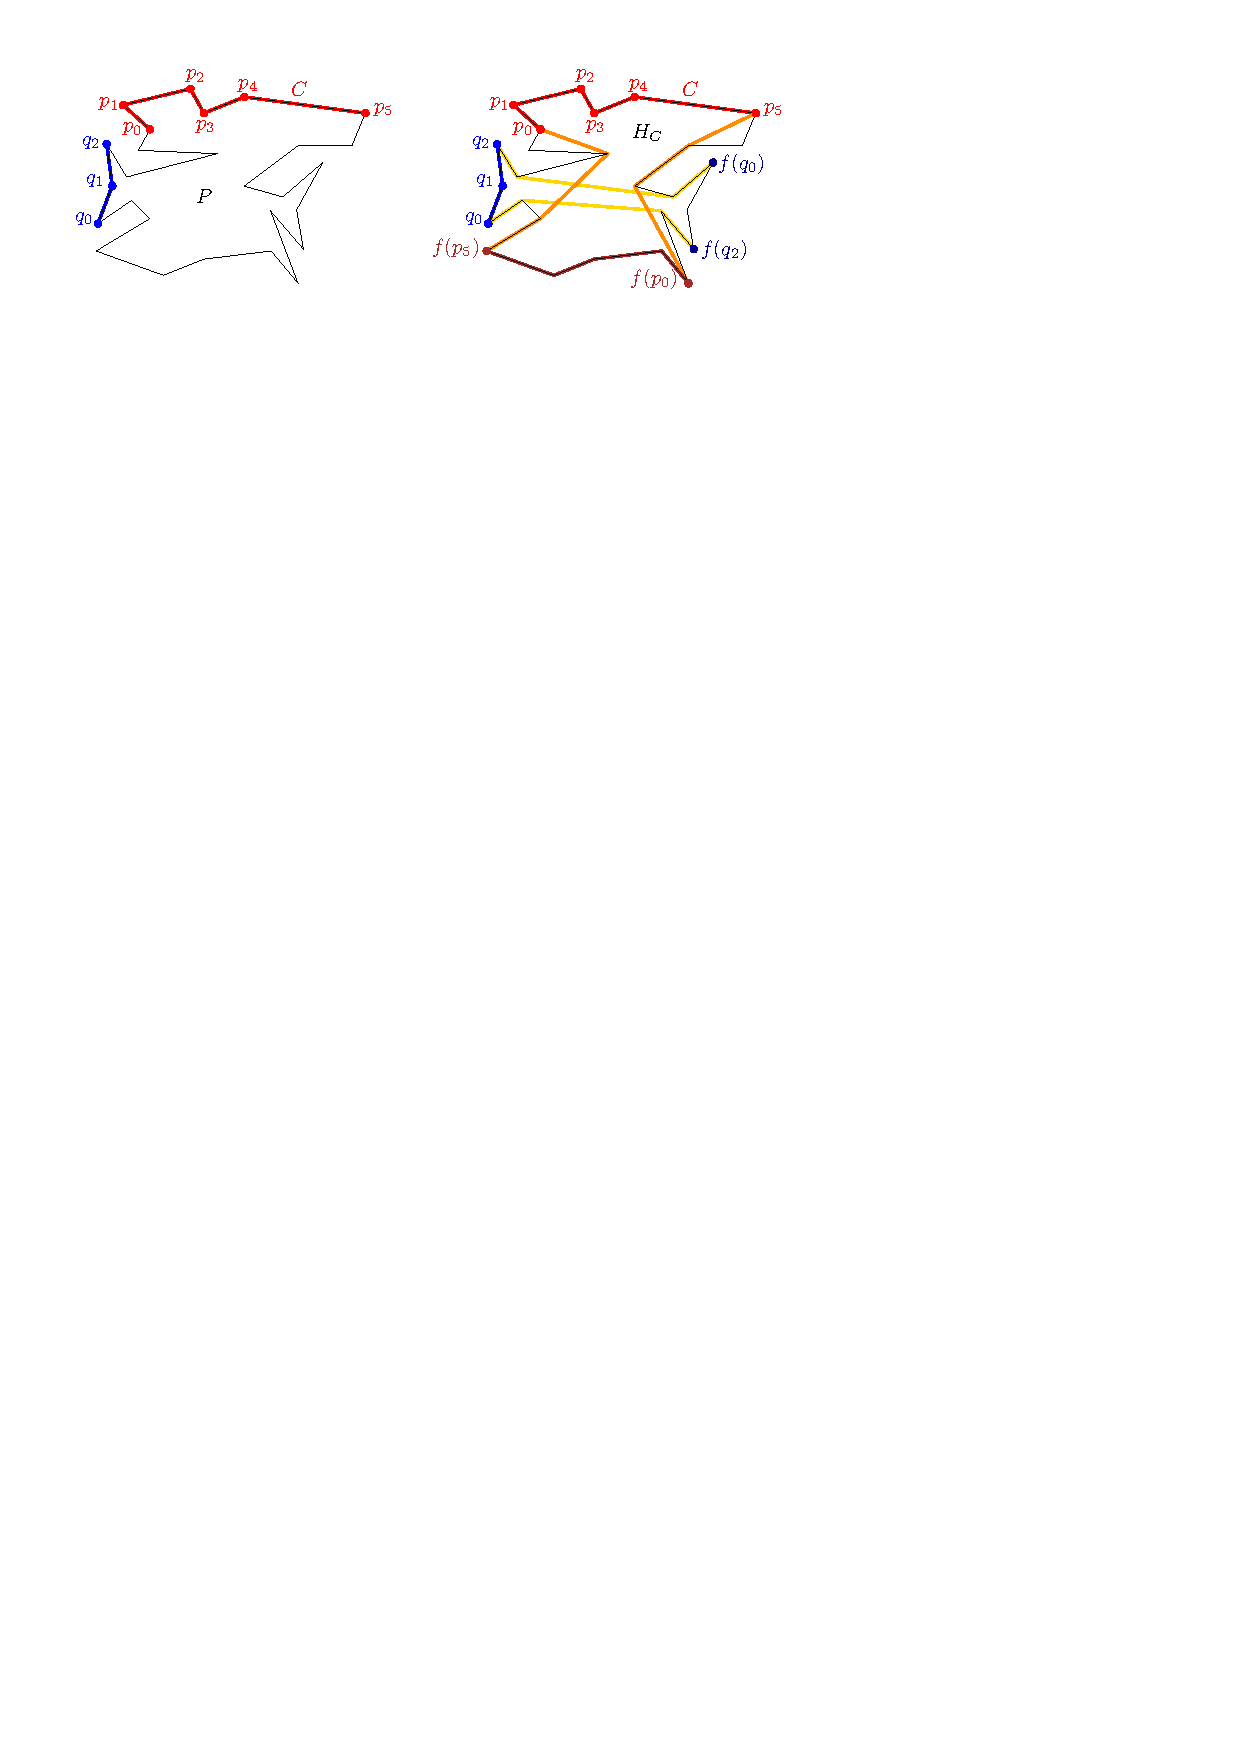
\includegraphics{img/TransitionChains.pdf}
\caption{\small }
\label{fig:Transition chains and hourglasses}
\end{figure}

We say that the hourglass $H_C$ is \emph{open} if its walls are vertex disjoint. 
We say $C$ is a \emph{transition chain} if $\ff{p_0} \neq \ff{p_k}$ and neither $\ff{p_0}$ nor $\ff{p_k}$ are interior vertices of $C$. In particular, if an edge $ab$ of $\partial P$ is a transition chain, we say that it is a \emph{transition edge}.

\begin{lemma}\label{lemma:Transition hourglasses are open}
[Rephrase of Lemma~3.1.3 of~\cite{aronov1993furthest}] 
If $C$ is a transition chain of $\partial P$, then the hourglass $H_C$ is an open hourglass.
\end{lemma}

Note that by Lemma~\ref{lemma:Transition hourglasses are open}, the hourglass of each transition chain is open.
In the remainder of the paper, all the hourglasses considered are defined by a transition chain, i.e., they are open and their top and bottom chain are edge disjoint.

The following results are similar or have already been proved by Suri~\cite{suri1989computing} and Aronov et al.~\cite{aronov1993furthest}. We provide a sketch of the proof of some of them for completeness.

The following lemma is depicted in Figure~\ref{fig:Order Lemma And Funnels} and is a direct consequence of the Ordering Lemma proved by Aronov et al.~\cite[Corollary 2.7.4]{aronov1993furthest}.
\begin{lemma}\label{lemma:Ordering Lemma}
Let $C_1, C_2, C_3$ be three edge disjoint transition chains of $\partial P$ that appear in this order when traversing clockwise the boundary of $P$. Then, the bottom chains of $H_{C_1}, H_{C_2}$ and $H_{C_3}$ are also edge disjoint and appear in this order when traversing clockwise the boundary of~$P$.
\end{lemma}

\begin{figure}[tb]
\centering
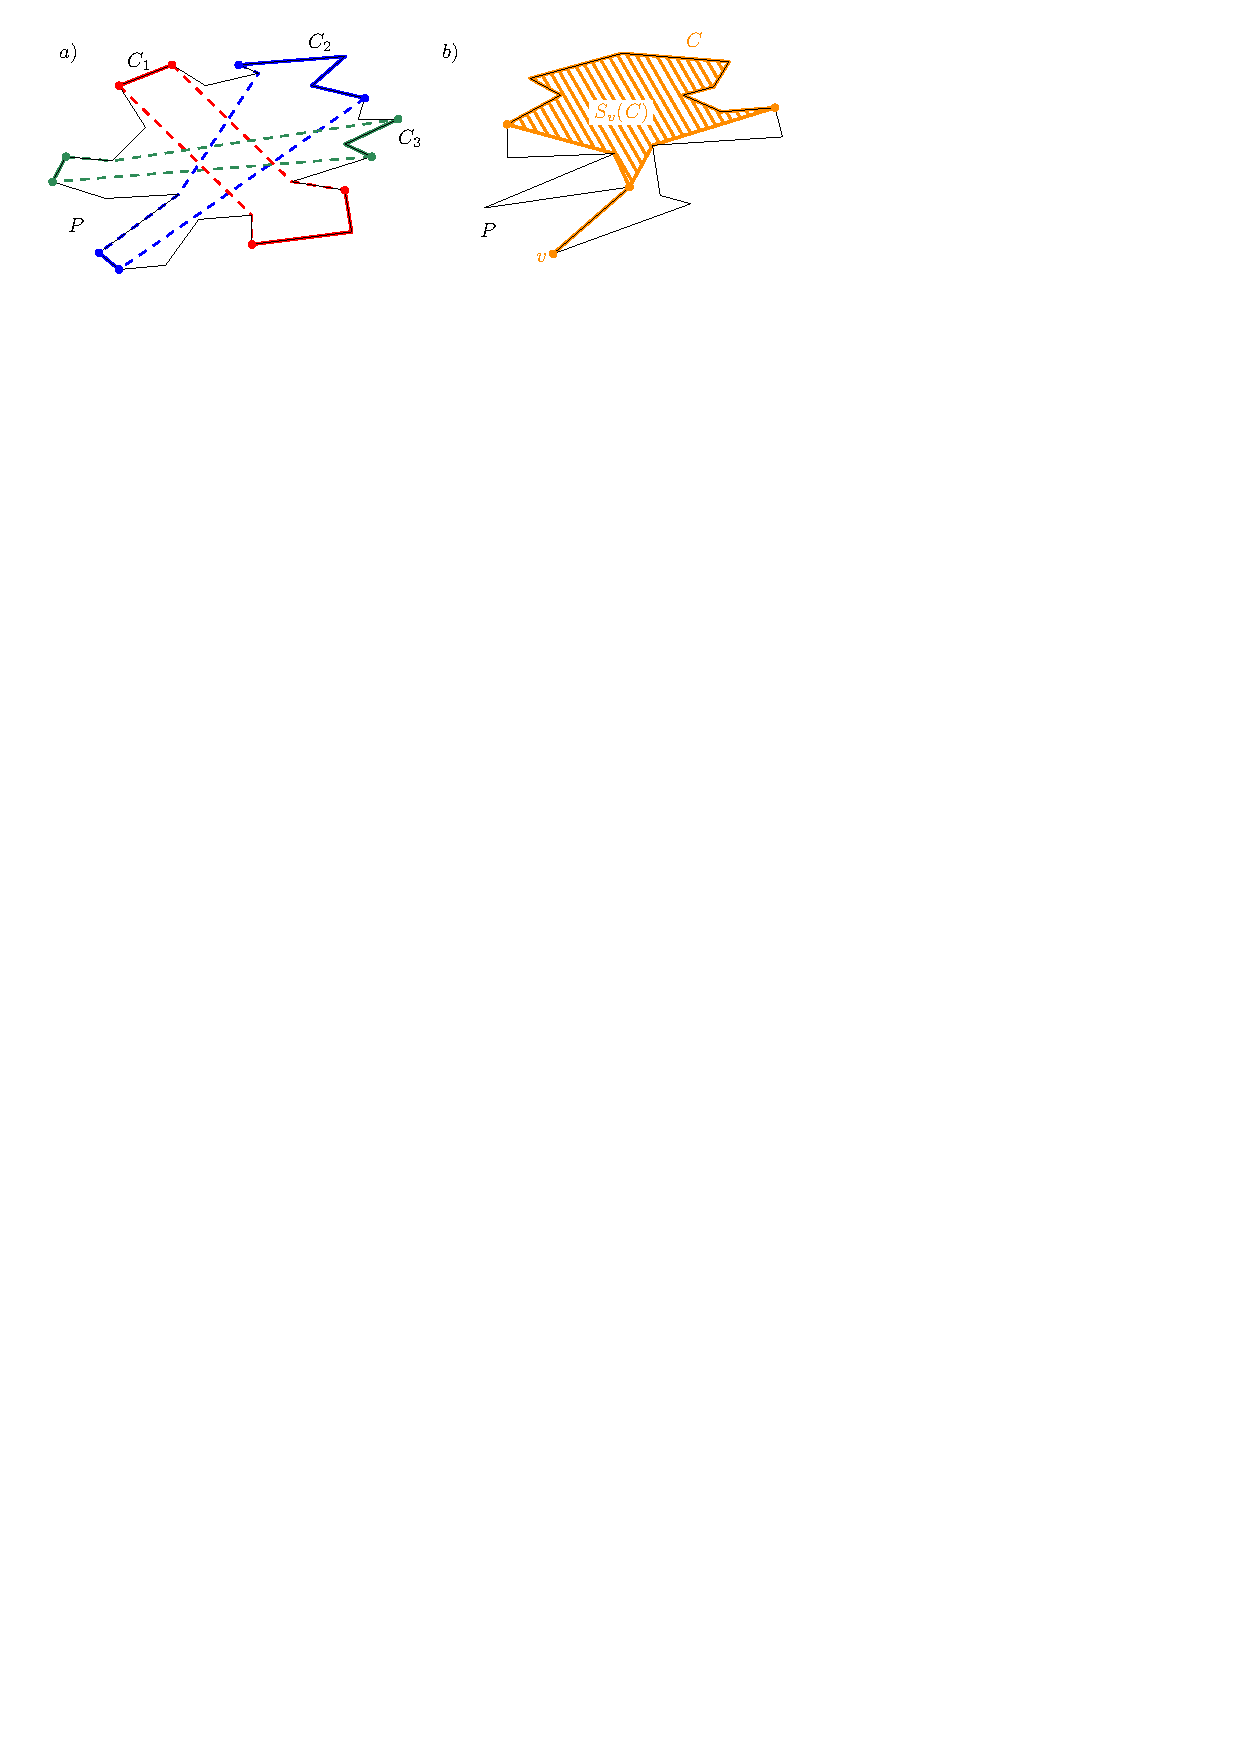
\includegraphics{img/OrderAndFunnel.pdf}

\caption{\small }
\label{fig:Order Lemma And Funnels}
\end{figure}


\begin{lemma}\label{lemma:Split paths}
Let $C_1, \ldots, C_r$ be a set of edge disjoint transition chains of $\partial P$ that appear in this order when traversing clockwise the boundary of $P$. Then there is a set of $t = O(1)$ geodesic paths $\gamma_1, \ldots, \gamma_t$ such that for each $1\leq i\leq r$ there exists $1\leq j\leq t$ such that $\gamma_j$ separates the top and bottom chains of $H_{C_i}$.
Moreover, this set can be computed in $O(n)$ time.
\end{lemma}
\begin{proof}
Aronov et al. showed that there exist four vertices $v_1, \ldots, v_4$ of $P$ and geodesic paths $\p{v_1}{v_2}, \p{v_2}{v_3}, \p{v_3}{v_4}$ such that for any point $x\in \partial P$, one of these paths separates $x$ from $\ff{x}$~\cite[Lemma 2.7.6]{aronov1993furthest}. Moreover, they show how to compute this set in $O(n)$ time.

Let $\Gamma= \{\p{v_i}{v_j} : 1\leq i < j\leq 4\}$ and note that $v_1, \ldots, v_4$ split the boundary of $P$ into at most four connected components.
If a chain $C_i$ is completely contained in one of this components, then one path of $\Gamma$ separates the top and bottom chain of $H_{C_i}$. Otherwise, some vertex $v_j$ is an interior vertex of $C_i$. However, because the chains $C_1, \ldots, C_r$ are edge disjoint, there are at most four chains in this situation. 
For each chain $C_i$ containing a vertex $v_j$, we add the geodesic path connecting the endpoints of $C_i$ to $\Gamma$.
Therefore, $\Gamma$ consists of $O(1)$ geodesic paths and each hourglass $H_{C_i}$ has its top and bottom chain separated by some path of $\Gamma$.
Since only $O(1)$ paths are computed, this can be done in linear time.
\end{proof}

A \emph{chord} of $P$ is an edge joining two non-adjacent vertices $a$ and $b$ of $P$ such that $ab\subseteq P$. Therefore, a chord splits $P$ into two sub-polygons.

\begin{lemma}\label{lemma:Edges appear a constant number of times}
[Rephrase of Lemma 3.4.3 of~\cite{aronov1993furthest}]
Let $C_1, \ldots, C_r$ be a set of edge disjoint transition chains of $\partial P$ that appear in this order when traversing clockwise the boundary of $P$. Then each chord of $P$ appears in $O(1)$ hourglasses among $H_{C_1}, \ldots, H_{C_r}$.
\end{lemma}
\begin{proof}
Assume for a contradiction that there is a chord $st$ that appears in three hourglasses $H_{C_i}, H_{C_j}$ and $H_{C_k}$ such that $1\leq i < j < k\leq r$. 
Note that chords can only appear on the walls of these hourglasses. Because the hourglasses are open, $st$ must be an edge on exactly one wall of each of these hourglasses. 

Assume that $s$ is visited before $t$ when going from the top to the bottom chain along these walls.
Let $\p{s_i}{t_i}$ be the wall of $S_i$ that contains $st$ such that $s_i$ and $t_i$ lie in the top and bottom chains of $H_{C_i}$, respectively. Define $\p{s_k}{t_k}$ analogously.

Because  $C_j$ lies in between $C_i$ and $C_k$, Lemma~\ref{lemma:Ordering Lemma} implies that the bottom chain of $C_j$ appears between the bottom chains of $C_i$ and $C_k$. Therefore, $C_j$ lies between $s_i$ and $s_k$ and the bottom chain of $H_{C_j}$ lies between $t_i$ and $t_k$. 
That is, for each $x\in C_j$ and each $y$ in the bottom chain of $H_{C_j}$, the geodesic path $\p{x}{y}$ is ``sandwiched'' by the paths $\p{s_i}{t_i}$ and $\p{s_k}{t_k}$.
Thus, $\p{x}{y}$ contains $st$.
However, this implies that the hourglass $H_{C_j}$ is not open---a contradiction that comes from assuming that $st$ lies in the  wall of three open hourglasses, when this wall is traversed from the top chain to the bottom chain. 
Analogous arguments can be used to bound the total number of walls that contain the edge $st$ (when traversed in any direction) to $O(1)$.
\end{proof}

%\begin{lemma}[Rephrase of Lemma 4 of~\cite{suri1989computing}]
%Let $C$ be a transition chain and let $B_C$ be the bottom chain of $H_C$. Let $x,y$ be two vertices such that $\p{x}{y}$ separates $C$ from $B_C$.  If $T_x$ and $T_y$ are the shortest-path trees of $x$ and $y$ in $P$, then for each $u\in C$ and each $v\in B_C$, all edges of $\p{u}{v}$, except perhaps one, belong to $T_x\cup T_y$.
%\end{lemma}

\begin{lemma}\label{lemma:Suri's lemma}
Let $x, u, y, v$ be four vertices of $P$ that appear in this cyclic order in a clockwise traversal of $\partial P$.
Given the shortest-path trees $T_x$ and $T_y$ of $x$ and $y$ in $P$, respectively, such that $T_x$ and $T_y$ can answer lowest common ancestor (LCA) queries in $O(1)$ time, 
we can compute the path $\p{u}{v}$ in $O(|\p{u}{v}|)$ time. 
Moreover, all edges of $\p{u}{v}$, except perhaps one, belong to $T_x\cup T_y$.
\end{lemma}
\begin{proof}
Let $X$ (\emph{resp.} $Y$) be the set containing the LCA in $T_x$ (\emph{resp.} $T_y$) of $u,y$, and of $v,y$ (\emph{resp.} $u,x$ and $x,y$).
Note that $X$ and $Y$ can be computed in $O(1)$ time.
Moreover, using LCA queries, we can decide their order along the path $\p{x}{y}$ when ordered from $x$ to $y$. Two cases arise: 

\textbf{Case 1.} If there is a vertex  $x^*\in X$ lying after a vertex $y^*\in Y$ in the order imprinted in $\p{x}{y}$, 
then the path $\p{u}{v}$ contains the path $\p{x^*}{y^*}$. 
In this case, the reader can verify that the path from $u$ to $v$ is contained in $T_x\cup T_y$. 
Moreover, it be computed in time proportional to its length by consider a couple of cases depending on which vertices defined $x^*$ and $y^*$; see Figure~\ref{fig:Output Sensitive Algorithm}.

\textbf{Case 2.} In this case both vertices of $X$ appear before the vertices of $Y$ along $\p{x}{y}$.
Let $x'$ (\emph{resp.} $y'$) be the vertex of $X$ (\emph{resp.} $Y$) closest to $x$ (\emph{resp.} $y$). 

Let $u'$ be the last vertex of $\p{u}{x}$ that is also in $\p{u}{y}$.
Note that $u'$ can be constructed by walking from $u'$ towards $x$ $y$ until the path towards $y$ diverges. 
Thus, $u'$ can be computed in $O(|\p{u}{u'}|)$ time. 
Define $v'$ analogously and compute it in $O(|\p{v}{v'}|)$ time.

Let $P'$ be the polygon bounded by the geodesic paths $\p{x'}{u'}, \p{u'}{y'}, \p{y'}{v'}$ and  $\p{v'}{x'}$.
Because the vertices of $X$ appear before those of $Y$ along $\p{x}{y}$, $P'$ is a simple polygon; see Figure~\ref{fig:Output Sensitive Algorithm}.

Note that the path $\p{u}{y}$ is the union of three paths $\p{u}{u'}, \p{u'}{v'}$ and $\p{v'}{v}$.
Because $\p{u}{u'}$ and  $\p{v'}{v}$ can be computed in time proportional to its length, it suffices to compute $\p{u'}{v'}$ in $O(|$\p{u'}{v'}$|)$ time.

Note that $P'$ is a simple polygon with only four convex vertices $x',u', y'$ and $v'$ connected by chains of reflex vertices. 
Regardless of the case, the shortest path from $x'$ to $y'$ can have at most one diagonal edge connecting distinct reflex chains of $P'$. Since the rest of the points in $\p{u'}{v'}$ lie on the boundary of $P'$ and from the fact that each edge of $P'$ is an edge of $T_x\cup T_y$, we conclude all edges of $\p{u}{v}$, except perhaps one, belong to $T_x\cup T_y$.

We want to find the common tangent between the reflex paths $\p{u'}{x'}$ and $\p{v'}{y'}$, or the common tangent of $\p{u'}{y'}$ and $\p{v'}{x'}$ as one of them belongs to the shortest path $\p{u'}{v'}$.
Assume that the desired tangent lies between the paths $\p{u'}{x'}$ and $\p{v'}{y'}$. 
Since this paths consist only of reflex vertices, the problem can be reduced to finding the common tangent of two convex polygons. By slightly modifying the trivial linear time algorithm, we can make it run in $O(|\p{u'}{v'}|)$ time. 

Since we do not know if the tangent lies between the paths $\p{u'}{x'}$ and $\p{v'}{y'}$, we process the chains $\p{u'}{y'}$ and $\p{v'}{x'}$ in parallel and stop when finding the desired tangent. Consequently, we can compute the path $\p{u}{v}$ in time proportional to ints length. 
\end{proof}

\begin{figure}[tb]
\centering
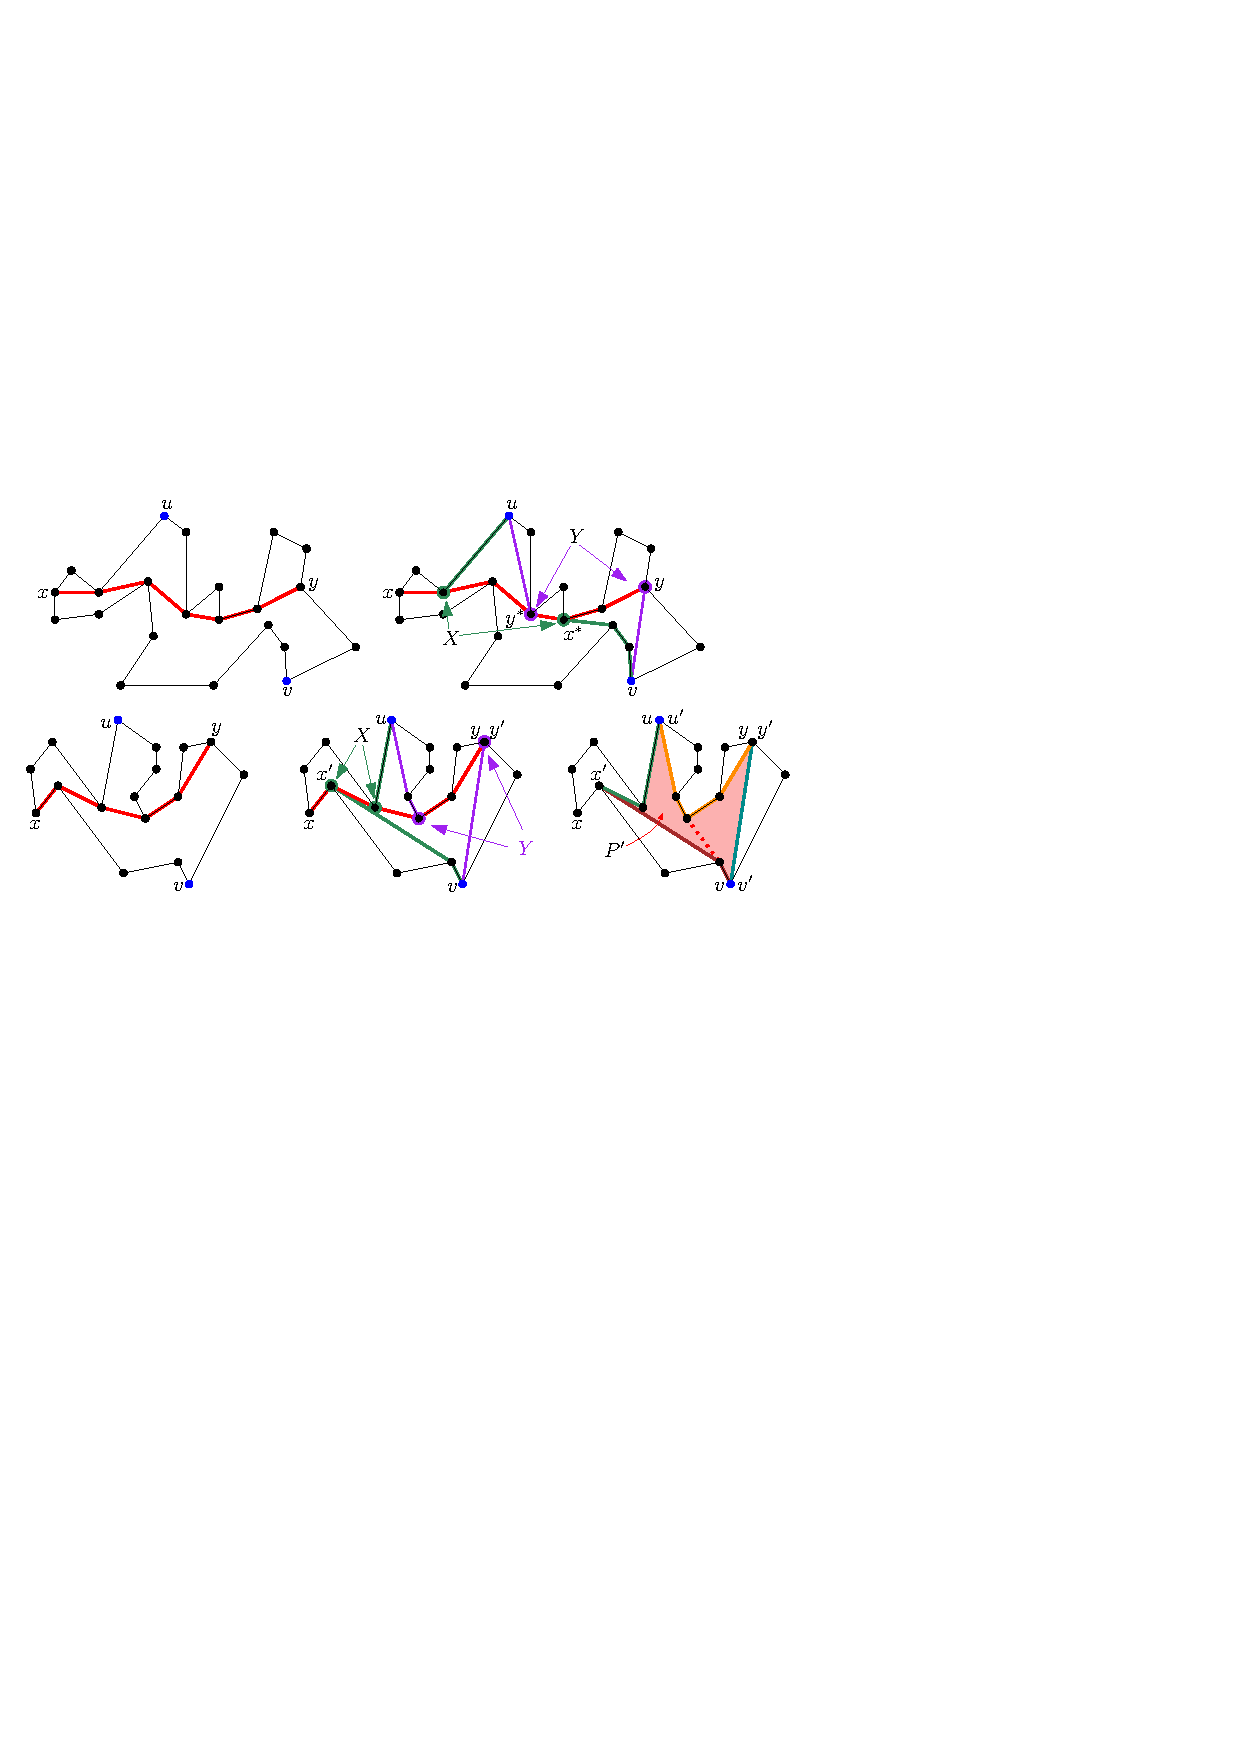
\includegraphics[width=1\textwidth]{img/OutputSensitive.pdf}

\caption{\small }
\label{fig:Output Sensitive Algorithm}
\end{figure}


\begin{lemma}\label{lemma:Bounding complexity of hourglasses}
Let $P$ be a simple polygon with $n$ vertices.
Given $k$ disjoint transition chains $C_1, \ldots, C_k$  of $\partial P$, it holds that  $$\sum_{i=1}^k |H_{C_i}| = O(n).$$
\end{lemma}
\begin{proof}

Because the given transition chains are disjoint, the bottom chains of their respective hourglasses are also disjoint by Lemma~\ref{lemma:Ordering Lemma}. Therefore, the sum of the complexities of all the top and bottom chains of these hourglasses amounts to $O(n)$. 
To bound the complexity of their walls, note that
Lemma~\ref{lemma:Edges appear a constant number of times} implies that no chord is used more that a constant number of times. Thus, it suffices to show that the total number of chords used by all these hourglasses is $O(n)$.

To prove this, we use Lemma~\ref{lemma:Split paths} to construct $O(1)$ \emph{split chains} $\gamma_1, \ldots, \gamma_t$ such that for each $1\leq i\leq k$, there is a split chain $\gamma_j$ that separates the top and bottom chain of $H_{C_i}$.
For each $1\leq j\leq t$, let $$\mathcal H^j = \{H_{C_i} : \text{the top and bottom chain of $H_{C_i}$ are separated by }\gamma_j\}.$$
Since the complexity of the shortest-path trees of the endpoints of $\gamma_j$ is $O(n)$~\cite{guibasShortestPathTree},
and from the fact that the chains $C_1, \ldots, C_k$ are disjoint,  Lemma~\ref{lemma:Suri's lemma} implies that
the total number of edges in all the hourglasses of $\mathcal H^j$ is $O(n)$. Moreover, because each of these edges appears in $O(1)$ hourglasses among $C_1, \ldots, C_k$, we conclude that 
$$\sum_{H \in \mathcal H^j } |H| = O(n).$$
Since we have only $O(1)$ split chains, our result follows.
\end{proof}

\subsection{Funnels}

Let $C = (p_0, \ldots, p_k)$ be a chain of the boundary of $P$ and let $v$ be a vertex of $P$ not in $C$.
The \emph{funnel} of $v$ to $C$, denoted by $\fn{v}{C}$, is the simple polygon bounded by $C$, $\p{p_k}{v}$ and $\p{v}{p_0}$; see Figure~\ref{fig:Order Lemma And Funnels}. 
Note that the paths $\p{v}{p_k}$ and $\p{v}{p_0}$ may coincide for a while before splitting into disjoint chains. 
See Lee and Preparata~\cite{lee1984euclidean} or Guibas et al.~\cite{guibasShortestPathTree} for more details on funnels.

A subset $R\subset P$ is \emph{geodesically convex} if for every $x,y\in R$, the path $\p{x}{y}$ is contained in $R$.
This funnel $\fn{v}{C}$ is also known as the geodesic convex hull of $C$ and $v$, i.e., the minimum geodesically convex set that contains $v$ and $C$.

Given two points $x,y\in P$, the (geodesic) \emph{bisector} of $x$ and $y$ is the set of points contained in $P$ that are equidistant from $x$ and $y$. This bisector is a curve, contained in $P$, that consists of circular arcs and hyperbolic arcs. Moreover, this curve intersects $\partial P$ only at its endpoints~\cite[Lemma 3.22]{aronov1989geodesic}.

\begin{lemma}\label{lemma:Funnel contains Voronoi cell}
Let $v$ be a vertex of $P$ and let $C$ be a transition chain such that $C$ contains $R(v)\cap \partial P$ and $v$ is not contained in $C$.
Then, $R(v)$ is contained in the funnel $\fn{v}{C}$
\end{lemma}
\begin{proof}
Let $a$ and $b$ be the endpoints of $C$ such that $a,b, \ff{a}$ and $\ff{b}$ appear in this order in a clockwise traversal of $\partial P$.
Because $R(v)\cap \partial P\subset C$, we know that $v$ lies between $\ff{a}$ and $\ff{b}$.

Let $\alpha$ (\emph{resp.} $\beta$) be the bisector of $v$ and $\ff{a}$ (\emph{resp.} $\ff{b}$).
Let $h_a$ (\emph{resp.} $h_b$) be the set of points of $P$ that are farther from $v$ than from $\ff{a}$ (\emph{resp.} $\ff{b}$).
Note that $\alpha$ is the boundary of $h_a$ while $\beta$ bounds $h_b$.

By definition, we know that $R(v)\subseteq h_a\cap h_b$. Therefore, it suffices to show that $h_a\cap h_b\subset \fn{v}{C}$.
Assume for a contradiction that there is a point of $h_a\cap h_b$ lying outside of $\fn{v}{C}$. 
By continuity, the boundaries of $h_a\cap h_b$ and $\fn{v}{C}$ intersect.
Because $a\notin h_a$ and $b\notin h_b$, both $\alpha$ and $\beta$ have an endpoint on the edge $ab$.
Since the boundaries of $h_a\cap h_b$ and $\fn{v}{C}$ intersect, we infer that $\beta \cap \p{v}{b}\neq \emptyset$ or $\alpha \cap \p{v}{a}\neq \emptyset$.
Without loss of generality, assume that there is a point $w\in \beta \cap \p{v}{b}$, the case where $w$ lies in $\alpha \cap \p{v}{a}$ is analogous. 

Since $w\in \beta$, we know that $\g{w}{v} = \g{w}{ \ff{b}}$. By the triangle inequality and since $w$ cannot be a vertex of $P$ as $w$ intersects $\partial P$ only at its endpoints, we get that
$$\g{b}{\ff{b}} < \g{b}{w} + \g{w}{\ff{b}} = \g{b}{w} + \g{w}{v} = \g{b}{v}.$$
Which implies that $b$ is farther from $v$ than from $\ff{b}$---a contradiction that comes from assuming that $h_a\cap h_b$ is not contained in $\fn{v}{C}$.
\end{proof}

\section{Decomposing the boundary}\label{Section:Decomposing the boundary}
In this section, we compute the farthest neighbor of each vertex of $P$. 
Note that the farthest neighbor of each vertex of $P$ is always a convex vertex of $P$~\cite{at-cgcsp-85}.

Using a result from Hershberger and Suri~\cite{hershberger1993matrix}, in $O(n)$ time we can compute the farthest neighbor of each vertex of $P$.
We then mark the vertices of $P$ that are farthest neighbors of at least one vertex of $P$.
Let $M$ denote the set of marked vertices of $P$ which can be computed in $O(n)$ time.
In other words, $M$ contains all vertices of $P$ whose Voronoi cell contains at least one vertex of $P$.

Given a vertex $v$ of $P$, the vertices of $P$ whose farthest neighbor is $v$ appear contiguously along $\partial P$~\cite{aronov1993furthest}. Therefore, after computing all this farthest neighbors, we effectively split the boundary into subchains, each associated with a different vertex of $M$; see Figure~\ref{fig:Marked vertices decomposition}.

\begin{figure}[tb]
\centering
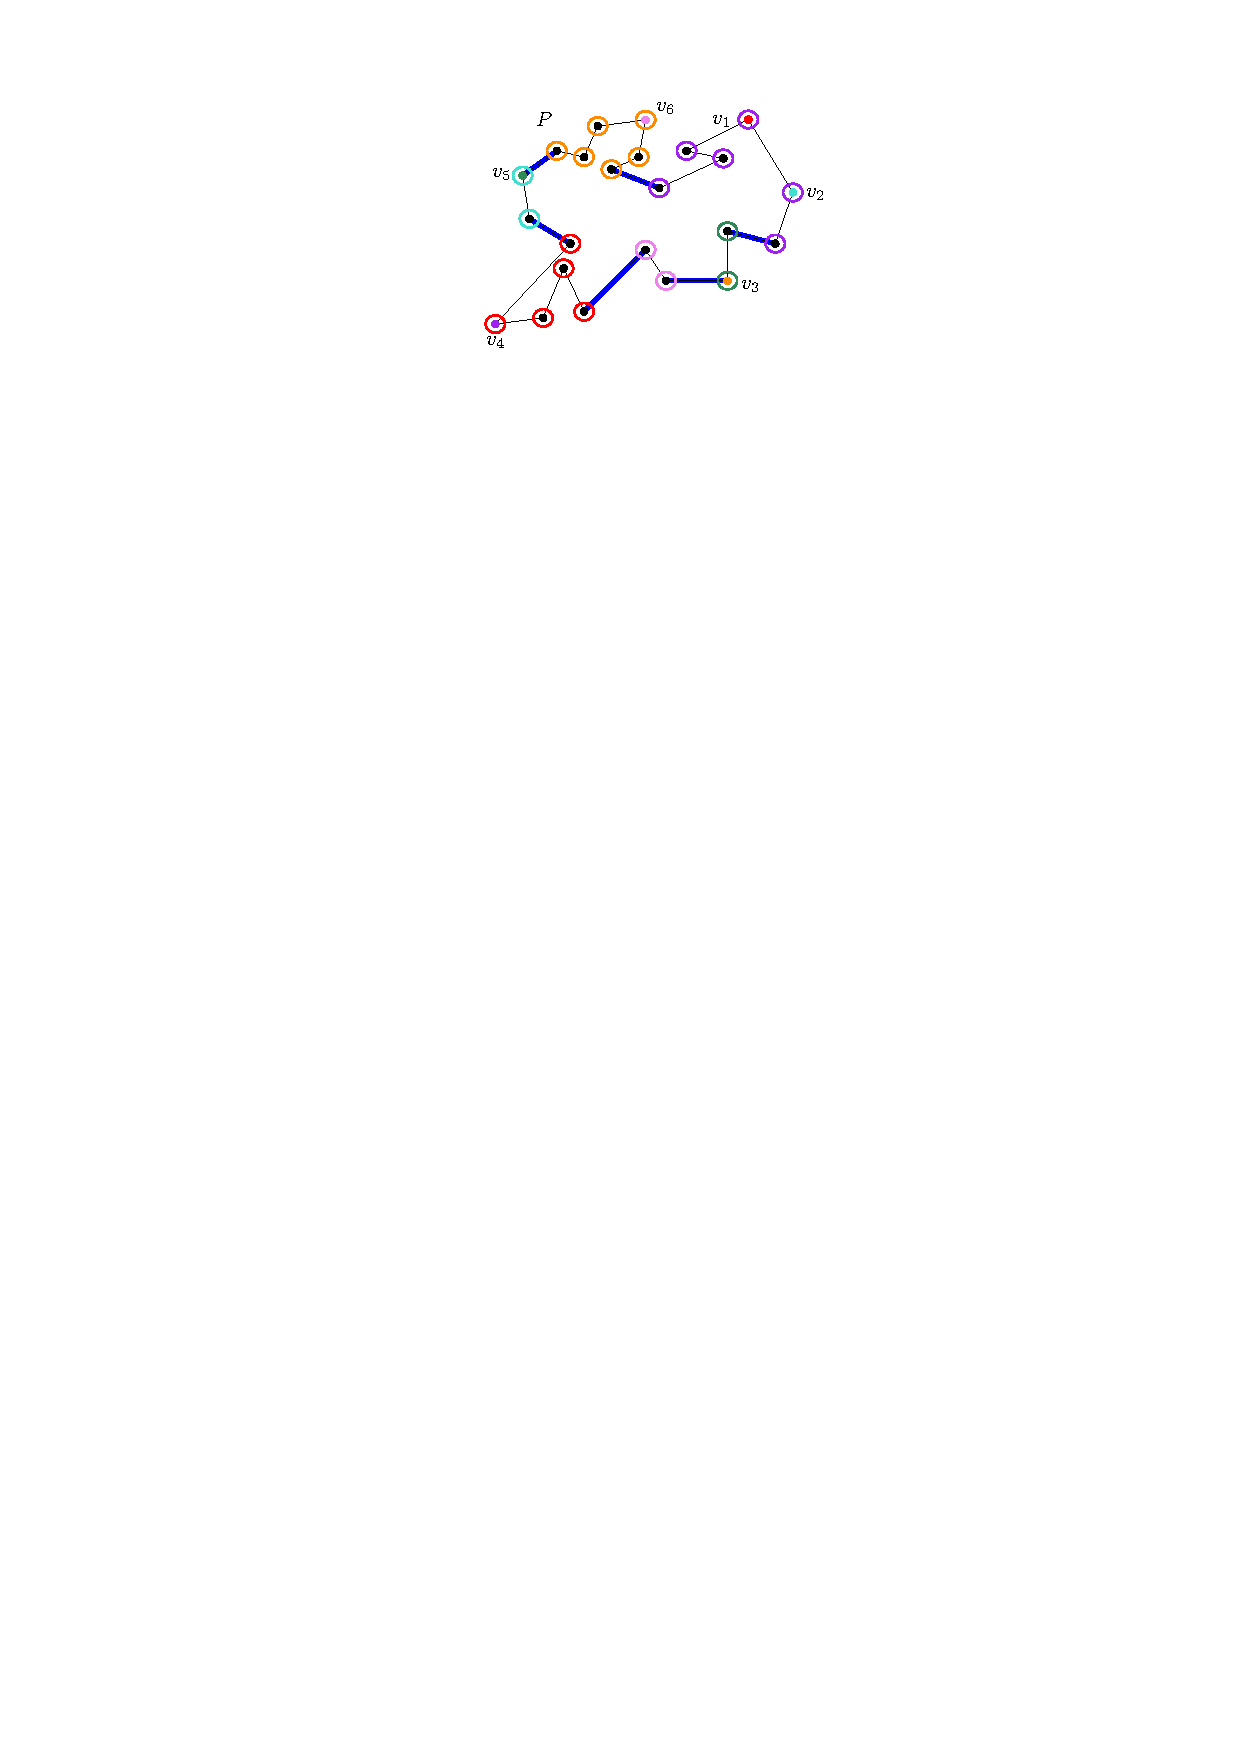
\includegraphics{img/MarkedVertices.pdf}

\caption{\small }
\label{fig:Marked vertices decomposition}
\end{figure}

Let $a$ and $b$ be the endpoints of a transition edge of $\partial P$ such that $a$ appears before $b$ in the clockwise order along $\partial P$. Because $ab$ is a transition edge, we know that $\ff{a}\neq \ff{b}$.
Recall that we have computed $\ff{a}$ and $\ff{b}$ in the previous step and note that $\ff{a}$ appears also before $\ff{b}$ along this clockwise order. 
For every vertex $v$ that lies between $\ff{a}$ and $\ff{b}$ in the bottom chain of $H_{ab}$, we know that there cannot be vertex $u$ of $P$ such that $\ff{u} = v$.
As proved by Aronov et al.~\cite[Corollary 2.7.4]{aronov1993furthest}, 
if there is a point $x$ on $\partial P$ whose farthest neighbor is $v$, then $x$ must lie on the open segment $(a,b)$. 
In other words, the Voronoi cell $R(v)$ restricted to $\partial P$ is contained in~$(a,b)$.

\section{Building hourglasses}\label{Section: Building hourglasses}

Let $E$ be the set of transition edges of $\partial P$.
Given a transition edge $ab\in E$, we say that $H_{ab}$ is a \emph{transition hourglass}.
In order to construct the triangle cover of $P$, 
we need to construct the transition hourglass of each transition edge of $E$.

By Lemma~\ref{lemma:Bounding complexity of hourglasses}, we know that $\sum_{ab\in E} |H_{ab}| = O(n)$.
Therefore, an output sensitive algorithm would suffice for this task. 
In this section, we present an algorithm that computes each transition hourglass of $P$ in $O(n)$ time.

Given a transition hourglass $H_{ab}$, we say that a geodesic path \emph{separates} $H_{ab}$ if it separates its top and bottom chains.
By Lemma~\ref{lemma:Split paths} we can compute a set of $O(1)$ separating paths such that for each transition edge $ab$, the transition hourglass $H_{ab}$ is separated by some path in this set.

Let $\gamma$ be a separating path whose endpoints are $x$ and $y$. 
Note that $\gamma$ separates the boundary of $P$ into two chains $S$ and $S'$ such that $S\cup S' = \partial P$.
Let $\mathcal H_S$ be the set of each transition hourglass separated by $\gamma$ whose transition edge is contained in $S$.
Note that $\mathcal H_S$ can be constructed in $O(n)$ time.
We claim that we can compute each transition hourglass of $\mathcal H_S$ in $O(n)$ time.
Note that the wall of each of these hourglasses consists of a (geodesic) path that connects a point in $S$ with a point in $S'$.

To compute these walls, we start by computing the shortest-path trees $T_x$ and $T_y$ of $x$ and $y$, respectively, in $O(n)$ time~\cite{guibasShortestPathTree}. Recall that there are $O(n)$ edges in total in both $T_x$ and $T_y$.

Let $u\in S$ and $v\in S'$ be two vertices such that $\p{u}{v}$ is the wall of a hourglass in $\mathcal H_S$.
By Lemma~\ref{lemma:Suri's lemma}, we can compute this path in $O(|\p{u}{v}|)$ time. 
Therefore, we can compute all hourglasses of $\mathcal H_S$ in $O(\sum_{H\in \mathcal H_S} |H| + n)$ time. 
Which amounts to $O(n)$ by Lemma~\ref{lemma:Bounding complexity of hourglasses}. 
Because there are only $O(1)$ separating paths by Lemma~\ref{lemma:Split paths}, we obtain the following result.

\begin{lemma}\label{lemma: Hourglass partition}
If $E$ is the set of transition edges of $P$, then we can construct the transition hourglass of each edge $E$ in total $O(n)$ time.
\end{lemma}

\section{Covering the polygon with apexed triangles}\label{Section:Computing apexed triangles}
An \emph{apexed triangle} $\triangle = (a,b,c)$ with \emph{apex} $a$ is a triangle contained in $P$ with an associated distance function $g_\triangle(x)$, called the \emph{apex function} of $\triangle$, such that (1) $a$ is a vertex of $P$, (2) $b$ and $c$ are points on the boundary of $P$, and (3) there is a  vertex $w$ of  $P$, called the \emph{definer} of $\triangle$, such that
$$g_\triangle(x) = \left\{ \begin{array}{lll}
-\infty&&\text{if $x\notin \triangle$}\\
|xa| + \g{a}{w} = \g{x}{w} && \text{if $x\in \triangle$}
\end{array}\right.$$

In this section, we show how to find a set of $O(n)$ apexed triangles of $P$ such that the upper envelope of their apex functions coincides with $\F{P}{x}$.
To this end, we first decompose the transition hourglasses into apex triangles that encode all the geodesic distance information inside them. Then, for each marked vertex $v\in M$, we construct a funnel that contains the Voronoi cell of $v$.  We then decompose this funnel into apex triangles that encode the distance from $v$.

\subsection{Inside the transition hourglass}
Let $ab$ be a transition edge of $P$  such that $b$ is the clockwise neighbor of $a$ along $\partial P$.
Let $B_{ab}$ denote the bottom chain of $H_{ab}$.
As noticed above, a point on $\partial P$ can be farthest from a vertex in $B_{ab}$ only if it lies in the open segment $ab$.
Formally, if $v$ is a vertex of $B_{ab}$ such that $R(v)\neq \emptyset$, then $R(v)\cap \partial P \subset ab$.
We claim that not only this Voronoi cell is inside $H_{ab}$ when restricted to the boundary of $P$, but that $R(v)\subset H_{ab}$. 

The next result follows trivially from Lemma~\ref{lemma:Funnel contains Voronoi cell}.

\begin{corollary}\label{lemma:Cell contained in geodesic triangle}
Let $v$ be a vertex of $B_{ab}$. If $R(v)\neq \emptyset$, then $R(v) \subset H_{ab}$.
\end{corollary}
%\begin{proof}
%Because $R(v)\cap \partial P \subset ab$, by Lemma~\ref{lemma:Funnel contains Voronoi cell}, we know that $R(v)\subset \fn{v}{ab}$. Because $H_{ab}$ is geodesically convex, we conclude that $R(v)\subset \fn{v}{ab}\subset H_{ab}$.
%\end{proof}
%%%


Our objective is to compute $O(|H_{ab}|)$ apexed triangles that cover $H_{ab}$, each with its distance function, such that the upper envelope of these apex functions coincides with $\F{P}{x}$ restricted to $H_{ab}$ where it ``matters''.

A similar approach was already carried on by Pollack et al. in~\cite[Section 3]{pollackComputingCenter}. 
Given a segment contained in the interior of $P$, they show 
how to compute a linear number of apexed triangles such that $\F{P}{x}$ coincides with the upper envelope of the corresponding apex functions in the given segment.

While the construction we follow is analogous, we use it in the transition hourglass $H_{ab}$ instead of the full polygon $P$. 
Therefore, we have to specify what is the relation between the upper envelope of the computed functions and $\F{P}{x}$. 
We will show that the upper envelope of the apex functions computed in $H_{ab}$ coincides with $\F{P}{x}$ inside the Voronoi cell $R(v)$ of every vertex $v\in B_{ab}$.

Let $T_a$ and $T_b$ be the shortest-path trees in $H_{ab}$ from $a$ and $b$, respectively. Assume that $T_a$ and $T_b$ are rooted at $a$ and $b$, respectively.
We can compute these trees in $O(|H_{ab}|)$ time~\cite{guibasShortestPathTree}. 
For each vertex $v$ between $\ff{a}$ and $\ff{b}$, let $v_a$ and $v_b$ be the neighbors of $v$ in the paths $\p{v}{a}$ and $\p{v}{ b}$, respectively.
We say that a vertex $v$ is \emph{visible} from $ab$ if $v_a\neq v_b$.
Note that if a vertex is visible, then the extension of these segments must intersect the top segment $ab$. 
Therefore, for each visible vertex $v$, we obtain a triangle $\triangle_v$ as shown in Figure~\ref{fig:Hourglass Cover}.

\begin{figure}[tb]
\centering
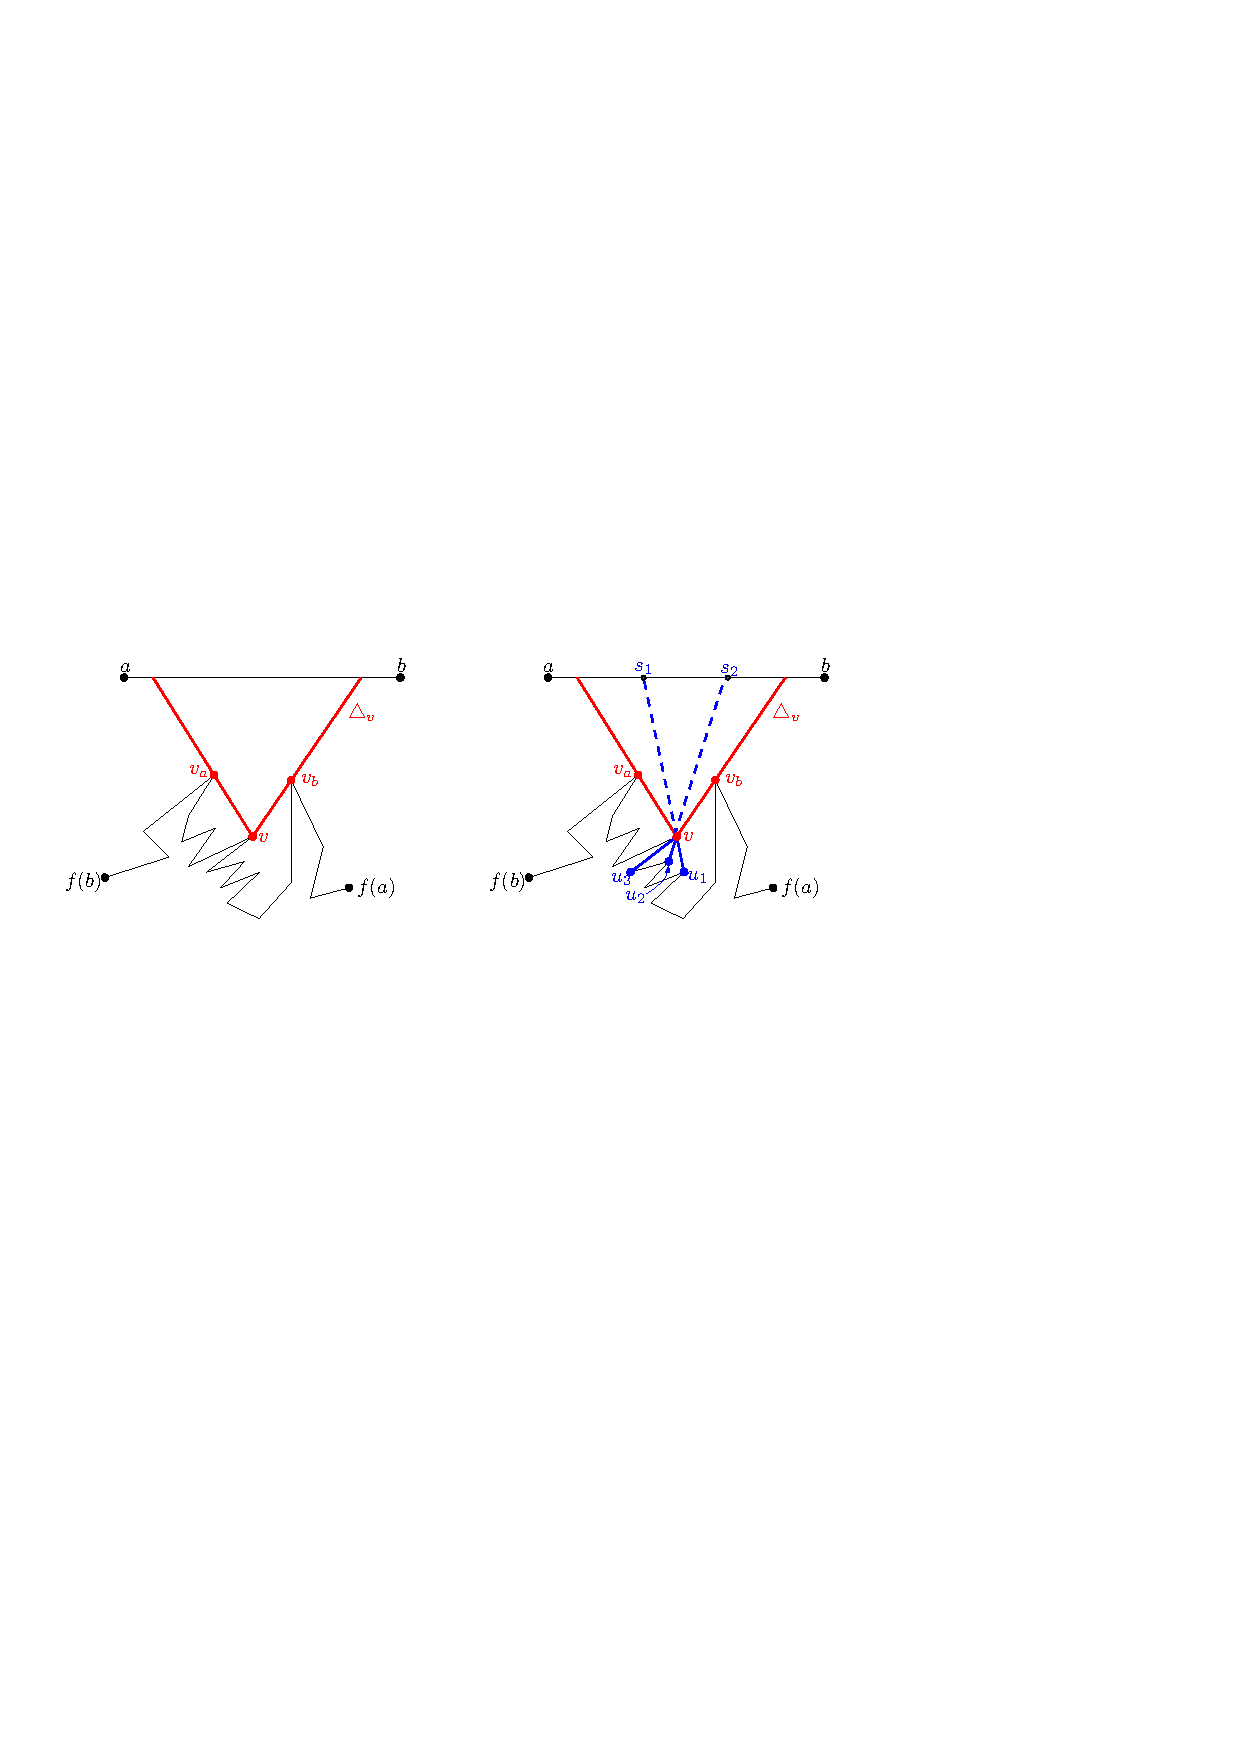
\includegraphics{img/HourglassCover.pdf}

\caption{\small }
\label{fig:Hourglass Cover}
\end{figure}

We further split $\triangle_v$ into a series of triangles with apex at $v$ as follows: 
Let $u$ be a child of $v$ in either $T_a$ or $T_b$. As noted by Pollack et al., $v$ can be of three types, either (1) $u$ is not visible from $ab$ (and is hence a child of $v$ in both $T_a$ and $T_b$); or (2) $u$ is visible from $ab$, is a child of $v$ only in $T_b$, and $v_b v u$ is a left turn; or (3) $u$ is visible from $ab$, is a child of $v$ only in $T_a$, and $v_a v u$ is a right turn.

Let $u_1, \ldots, u_{k-1}$ be the children of $v$ of type $(2)$ sorted in clockwise order around $v$.
Let $c(v)$ be the maximum distance from $v$ to any invisible vertex in the subtrees of $T_a$ and $T_b$ rooted at $v$; if no such vertex exists, then $c(v) = 0$. 
Define a function $d_l(v)$ on each vertex $v$ of $H_{ab}$ in a recursive fashion as follows:
If $v$ is invisible from $ab$, then $d_l(v) = c(v)$. 
Otherwise, let $d_l(v)$ be the maximum of $c(v)$ and $\max\{d_l(u_i) + |u_iv| : u_i$ is a child of $v$ of type $(2)\}$.
Similarly we define a symmetric function $d_r(v)$ using the children of type (3) of $v$.

For each $1\leq i\leq k-1$, extend the segment $u_iv$ past $v$ until it intersects $ab$ at a point $s_i$. Let $s_0$ and $s_k$ be the intersections of the extensions of $vv_a$ and $vv_b$ with the segment $ab$.
We define then $k$ triangles contained in $\triangle_v$ as follows. 
For each $0\leq i\leq k-1$, consider the triangle $\triangle(s_i, v, s_{i+1})$ whose associated apexed (left) function is 
$$f_i(x) = |xv| + \max_{j>i}\{c(v), |vu_j| + d_l(u_j)\}.$$
In a symmetric manner, we define a set of apexed triangles induced by the type (3) children of~$v$ and their respective apexed (right) functions.

Let $g_1, \ldots, g_r$ and $\triangle_1, \ldots, \triangle_r$ respectively be an enumeration of all the generated apex functions and triangles such that $g_i$ is defined in the triangle $\triangle_i$. Because each function is determined uniquely by a pair of adjacent vertices in $T_a$ or in $T_b$, and since these trees have $O(|H_{ab}|)$ vertices, we conclude that $r = O(|H_{ab}|)$. 

Note that for each $1\leq i\leq r$, the triangle $\triangle_i$ has two vertices on the segment $ab$ and a third vertex, say $a_i$, called its \emph{apex} such that for each $x\in \triangle_i$, $g_i(x) = \g{x}{w_i}$ for some vertex $w_i$ of $H_{ab}$. We refer to $w_i$ as the \emph{definer} of $\triangle_i$. Intuitively, $\triangle_i$ defines a portion of the geodesic distance function from $w_i$ in a constant complexity region. 

\begin{lemma}\label{lemma:Triangles inside hourglasses}
Given a transition edge $ab$ of $P$, we can compute a set $\mathcal A_{ab}$ of $O(|H_{ab}|)$ apexed triangles in $O(|H_{ab}|)$ time with the property that for any point $p\in P$ such that $\ff{p}\in B_{ab}$,
there is an apexed triangle $\triangle\in \mathcal A_{ab}$ with apex function $g$ and definer equal to $\ff{p}$ such that
\begin{enumerate}
\item $p\in \triangle$ and 
\item $g(p) = \F{P}{p}$.
\end{enumerate}
\end{lemma}
\begin{proof}
Because $p\in R(\ff{p})$, Lemma~\ref{lemma:Cell contained in geodesic triangle} implies that $p\in H_{ab}$. 
Consider the path $\p{p}{\ff{p}}$ and let $v$ be the neighbor of $p$ along this path. 
Note that by construction, there is a triangle $\triangle\in \mathcal A_{ab}$ apexed at $v$ with definer $w$ that contains $p$. 
Recall that by construction, the apex function $g(x)$ of $\triangle$ encodes the geodesic distance from $x$ to $w$. 
Because $\F{P}{x}$ is the upper envelope of all the geodesic functions, we know that $g(p) \leq \F{P}{p}$.

To prove the other inequality, note that if $v = \ff{p}$, then trivially $g(p) = |pv| + \g{v}{w} \geq |pv| = \g{p}{\ff{p}} = \F{P}{p}$. 
Otherwise, let $z$ be the next vertex after $v$ in the path $\p{p}{\ff{p}}$. Three cases arise:

($a$) If $z$ is invisible from $ab$, then so is $\ff{p}$ and hence, 
$$\g{p}{ \ff{p}} = |pv| + \g{v}{ \ff{p}} \leq |pv| + c(v) \leq g(p).$$

($b$) If $z$ is a child of type (2), then $z$ plays the role of some child $u_j$ of $v$ in the notation used during the construction.
In this case:
$$\g{p}{\ff{p}} = |pv| + |v z| + \g{z}{\ff{p}} \leq |pv| + |v u_j| + d_l(u_j) \leq g(p).$$

($c$) If $z$ is a child of type (3), then analogous arguments hold using the (right) distance~$d_r$.

Therefore, regardless of the case $\F{P}{p} = \g{p}{ \ff{p}} \leq g(p)$.

To bound the running time, note that the recursive functions $d_l, d_r$ and $c$ can be computed in $O(|T_a| + |T_b|)$ time. Then, for each vertex visible from $ab$, we can process it in time proportional to its degree in $T_a$ and $T_b$.
Because the sum of the degrees of all vertices in $T_a$ and $T_b$ is $O(|T_a| + |T_b|)$ and from the fact that both $|T_a|$ and $|T_b|$ are $O(|H_{ab}|)$, we conclude that the total running time to construct $\mathcal A_{ab}$ is $O(|H_{ab}|)$.
\end{proof}

In other words, Lemma~\ref{lemma:Triangles inside hourglasses} says that by considering the apex functions of the apexed triangle in $\mathcal A_{ab}$, we do not lose any information inside any region $R(v)$ of any vertex $v\in B_{ab}$.

Following the same intuition, in the next section we construct a set of apexed triangles, and their apex functions, encoding the distance from the vertices of $M$.

\subsection{Inside the funnels of marked vertices}
Recall that for each marked vertex $v\in M$, we know at least of one vertex on $\partial P$ such that $v$ is its farthest neighbor.
Let $u_1, \ldots, u_{k-1}$ be the set of vertices of $P$ such that $v = \ff{u_i}$ and assume that they appear in this order when traversing $\partial P$ clockwise. Let $u_0$ and $u_k$ be the neighbors of $u_1$ and $u_{k-1}$ other than $u_2$ and $u_{k-2}$, respectively. Note that both $u_0 u_1$ and $u_{k-1}u_k$ are transition edges of $P$. Thus, we can assume that their transition hourglasses have been computed.

Let $C_v = (u_0, \ldots, u_k)$ and consider the funnel $\fn{v}{C_v}$.
We call $C_v$ the \emph{main chain} of $\fn{v}{C_v}$ while $\p{u_k}{ v}$ and $\p{v}{ u_0}$ are referred to as the \emph{walls} of the funnel.  
Because $v = \ff{u_0} = \ff{u_{k-1}}$, we know that $v$ is a vertex of both $H_{u_0 u_1}$ and  $H_{u_{k-1}u_k}$. 
Thus, since $\p{v}{ u_0}\subset H_{u_0u_1}$ while $\p{v}{u_k}\subset H_{u_{k-1}u_k}$, we can compute both $\p{v}{ u_0}$ and $\p{v}{u_k}$ in $O( |H_{u_0 u_1}| + |H_{u_{k-1}u_k}|)$ time.
Consequently, the funnel $\fn{v}{C_v}$ can be constructed in $O(k + |H_{u_0 u_1}| + |H_{u_{k-1}u_k}|)$. 

Because a vertex on $\partial P$ has a unique farthest neighbor by our general position assumption, and since the total sum of the complexities of the transition hourglasses is $O(n)$ by Lemma~\ref{lemma:Bounding complexity of hourglasses}, we can compute the funnel of each vertex of $M$ in total $O(n)$ time. 

Since the complexity of the walls of these funnels is bounded by the complexity of the transition hourglasses used to compute them, we get that $$\sum_{v\in M} |\fn{v}{C_v}|  = O\left(n + \sum_{ab\in E} |H_{ab}|\right) = O(n).$$

\begin{lemma}\label{lemma:Farthest points from marked are in funnel}
Let $x$ be a point in $P$. If $v = \ff{x}$, then $x\in \fn{v}{C_v}$.
\end{lemma}
\begin{proof}
Because $\ff{u_0} \neq \ff{u_k}$, we know that $C_v$ is a transition chain. Moreover, $C_v$ contains $R(v)\cap \partial P$ by definition. Therefore, by Lemma~\ref{lemma:Funnel contains Voronoi cell}, we know that $R(v)\subset \fn{v}{C_v}$.
Since $v = \ff{x}$, we know that $x\in R(v)$ and hence that $x \in \fn{v}{C_v}$. 
\end{proof}

Given a funnel $\fn{v}{C_v}$, we would like to split it into $O(|\fn{v}{C_v}|)$ apexed triangles that encode the distance function from $v$.
To this end, we compute the shortest-path tree $T_v$ of $v$ in $\fn{v}{C_v}$ in $O(|\fn{v}{C_v}|)$ time~\cite{guibasShortestPathQueries}.
We consider the tree $T_v$ to be rooted at $v$ and assume that for each node $u$ of this tree 
we have stored the geodesic distance $\g{u}{v}$. 

Let $w_1$ be the first leaf of $T_v$ found when walking from $v$ around $T_v$ in clockwise order as in an Eulerian tour.
Continue this Eulerian tour from $w_1$ and let $w_2$ and $w_3$ be the next two vertices visited. Two cases arise:

\textbf{Case 1.} If $w_1, w_2, w_3$ makes a left turn, then if $w_1$ and $w_3$ are adjacent, then construct an apexed triangle $\triangle(w_1, w_2, w_3)$ apexed at $w_2$ with apex function $g(x) = |x w_2| + \g{w_2}{v}$.
Otherwise, let $s$ be the first point of the boundary of $\fn{v}{C_v}$ hit by the ray shooting from $w_3$ in the direction opposite to $w_2$ ($s$ could be equal to $w_3$ if $w_3$ already lies on the boundary).

We claim that $s$ and $w_1$ lie on the same edge of the boundary of $\fn{v}{C_v}$. 
Otherwise, there would be a vertex $u$ visible from $w_2$ inside the wedge with apex $w_2$ spanned by $w_1$ and $w_3$.
Note that the first edge of the path $\p{u}{v}$ is the edge $uw_2$. Therefore, $uw_2$ belongs to the shortest-path $T_v$ contradicting the Eulerian order in which the vertices of this tree are visited as $u$ should be visited before $w_3$. Thus, $s$ and $w_1$ lie on the same edge and $s$ can be computed in $O(1)$ time.
We then construct an apexed triangle $\triangle(w_1, w_2, s)$ apexed at $w_2$ with apex function $g(x) = |x w_2| + \g{w_2}{v}$.
We now modify the tree $T_v$ by removing the edge $w_1w_2$ and adding the edge $w_3s$ (no edge is added if $w_3 = s$); see Figure~\ref{fig:Funnel Cover} for an illustration.

\begin{figure}[tb]
\centering
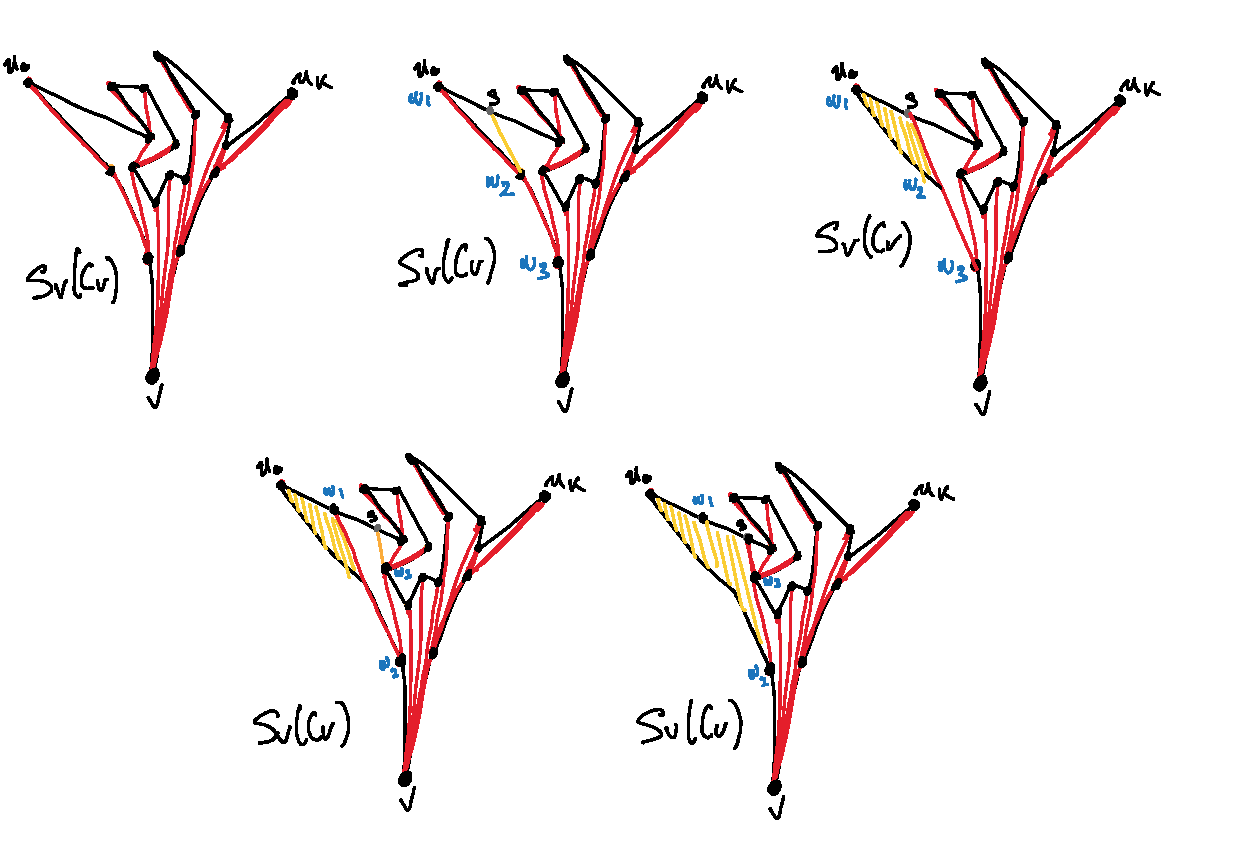
\includegraphics{img/FunnelCover.pdf}

\caption{\small }
\label{fig:Funnel Cover}
\end{figure}

\textbf{Case 2.} If $w_1, w_2, w_3$ makes a right turn, then let $s$ be the first point hit by the ray apexed at $w_2$ that shoots in the direction opposite to $w_3$. By the same argument as above, we can show that $w_1$ and $s$ lie on the same edge of the boundary of $\fn{v}{C_v}$. Therefore, we can compute $s$ in $O(1)$ time. At this point, we construct the apexed triangle $\triangle(w_1, w_2, s)$ apexed at $w_2$ with apex function $g(x) = |x w_2| + \g{w_2}{v}$.
We now modify the tree $T_v$ by removing the edge $w_1w_2$ and replacing the edge $w_3w_2$ by the edge $w_3s$; see Figure~\ref{fig:Funnel Cover}.

\begin{lemma}\label{lemma:Triangles inside funnels}
The above procedure runs in $O(|\fn{v}{C_v}|)$ time and computes $O(|\fn{v}{C_v}|)$ interior disjoint apexed triangles such that their union covers $\fn{v}{C_v}$. Moreover, for each point $x\in \fn{v}{C_v}$, there is an apexed triangle $\triangle$ with apex function $g(x)$ such that (1) $x\in \triangle$ and (2) $g(x) = \g{x}{v}$.
\end{lemma}
\begin{proof}
The above procedure splits $\fn{v}{C_v}$ into apexed triangles, such that the apex function in each of them is defined as the geodesic distance to $v$. Since the path towards $v$ of every point in these triangles has to go through their apex, we obtain properties (1) and (2).

To bound the running time and complexity we proceed as follows. 
We can compute the shortest-path tree $T_v$ from $v$ in $O(|\fn{v}{C_v}|)$ time~\cite{guibasShortestPathTree}.
Note that processing either Case 1 or 2 of the algorithm takes constant time. Therefore, we are only interested in the number of times these steps are performed. Note that we are removing a leaf of the tree in each iteration. In Case 2, the number of leaves strictly decreases, while in case one a new leaf is added if $s\neq w_3$. However, the number of leaves that can be added is at most the number of edges of $T_v$. Note that the edges added by either Case 1 or 2 are chords of the polygon and hence cannot generate further leaves. Because $|T_v| = O(|\fn{v}{C_v}|)$, we conclude that either Case 1 or 2 is only executed $O(|\fn{v}{C_v}|)$ times yielding the bound in the number of produced apexed triangles and in the running time.
\end{proof}

\section{Prune and search}\label{section:Prune and search}

In this section, we describe a procedure that finds either the geodesic center of $P$, or a convex trapezoid that contains the geodesic center.
The idea of the proof is to consider the chords of the apexed triangles computed in previous sections and use a cutting of them that splits $P$ into $O(1)$ cells. Then, we test on which cell the geodesic center lies and recurse on that cell as a new subproblem having smaller complexity. To decrease the complexity of the problem, we consider only the apexed triangles intersecting this cell in the next iteration. Using the properties of the cutting, we are able to prove that the size of the subproblem decreases by a constant fraction which leads to a linear running time. This algorithm has however two stopping conditions, one is to reach a subproblem of constant size, and a second one is to find a convex trapezoid containing the geodesic center. In the latter case, we are not able to proceed with the prune and search. Nevertheless, by restricting the search space to a convex object, we are able to perform standard optimization techniques to find the geodesic center.


Let $\tau$ be the set all apexed triangles computed in previous sections. 

\begin{lemma}\label{lemma:Size of tau}
The set $\tau$ consists of $O(n)$ apexed triangles.
\end{lemma}
\begin{proof}
To bound the complexity of $\tau$, recall that $E$ denotes the set of transition edges of $P$.
Because $\sum_{ab\in E} H_{ab} = O(n)$ by Lemma~\ref{lemma:Bounding complexity of hourglasses} and since there are $O(|H_{ab}|)$ apexed triangles in each transition hourglass $H_{ab}$, we conclude that there $O(n)$ apexed triangles constructed using Lemma~\ref{lemma:Bounding complexity of hourglasses}.

Furthermore, we know that $\sum_{v\in M} |\fn{v}{C_v}| = O(n)$. Because each funnel $\fn{v}{C_v}$ is subdivided into $O(|\fn{v}{C_v}|)$ apexed triangles by Lemma~\ref{lemma:Triangles inside funnels}, we conclude that at most $O(n)$ apexed triangles area constructed inside funnels of marked vertices. Consequently $|\tau| = O(n)$.
\end{proof}




Let $\phi(x)$ be the upper envelope of the apex functions of every triangle in $\tau$, i.e., $$\phi(x) = \max\{g(x) : g(x)\text{ is the apex function of some apexed triangle of }\tau\}.$$
The following result shows that the $O(n)$ apexed triangle of $\tau$ not only cover $P$, but their apex functions suffice to reconstruct the function $\F{P}{x}$.

\begin{lemma}\label{lemma:Optimization problem same as geodesic center}
The functions $\phi(x)$ and $\F{P}{x}$ coincide in the domain of points of $P$, i.e., for each $p\in P$, $\phi(p) = \F{P}{p}$.
\end{lemma}
\begin{proof}
Let $p$ be a point in $P$, we want to prove that $\phi(p) = \F{P}{p}$. 
Two cases arise: 
\textbf{Case 1.} If $\ff{p}$ is a marked vertex, then Lemma~\ref{lemma:Farthest points from marked are in funnel} implies that $p\in \fn{\ff{p}}{C_{\ff{p}}}$. Therefore
by Lemma~\ref{lemma:Triangles inside funnels} there is an apexed triangle $\triangle$ with apex function $g(x)$ such that $p\in \triangle$ and $g(p) = \g{p}{\ff{p}} = \F{P}{p}$.

\textbf{Case 2.} If $\ff{p}$ is not marked, then it belongs to the bottom chain of some transition hourglass. In this case by Lemma~\ref{lemma:Triangles inside hourglasses} there is an apexed triangle $\triangle$ with apex function $g(x)$ such that $p\in \triangle$ and $g(p) = \F{P}{p}$.

Regardless of the case, there is an apexed triangle $\triangle$ that contains $p$ such that its apex function $g(p) = \F{P}{p}$.
Since each apex function represent the geodesic distance from some vertex of $P$, we know that $\phi(p) \leq \F{P}{p}$. Moreover, since $g(x)$ is an apex function, we know that $g(p) \leq \phi(p)$.
Because $g(p) = \F{P}{p}$ and since $g(p) \leq \phi(p) \leq  \F{P}{p}$, we conclude that $\phi(p) = \F{P}{p}$ proving our claim.
\end{proof}


A \emph{$P$-chain} is a polygonal chain contained in the boundary of $P$.
A \emph{$P$-cell} is a simple polygon contained in $P$ bounded by a $P$-chain and a polygonal chain of length at most four contained in the interior of $P$ that connects the endpoints of this $P$-chain. Moreover, a $P$-cell contains the geodesic center of $P$.
The recursive algorithm described in this section takes as input a $P$-cell (originally the whole polygon $P$) and the set of apexed triangles of $\tau$ that intersect this $P$-cell, and produces then a new $P$-cell of smaller complexity.

Given a $P$-cell $R$, let $\tau_R$ be the set of apexed triangles of $\tau$ that intersect $R$.
Let $R$ be a $P$-cell and assume that the set $\tau_R$ has been computed.
Let $m = \max\{|R|, |\tau_R|\}$.

Note that each triangle of $\tau_R$ consists of at least one chord of $R$.
Let $C$ be the set containing all chords that bound a triangle of $\tau_R$. 
A \emph{half-chord} of $R$ is either of the simple polygons in which a chord of $R$ splits this polygon.
An \emph{$R$-trapezoid} is the simple polygon obtained as the intersection of at most four half-chords.
Consider a set $Q$ of all open $R$-trapezoids. 
For each $q\in Q$, let $C_q = \{c\in C: c\cap q \neq \emptyset\}$ be the set of chords of $C$ induced by $q$. 
Finally, let $Q_C = \{C_q : q\in Q\}$ be the family of subsets of $C$ induced by $Q$.

Consider the range space defined by $C$ and $F_C$. 
Let $\varepsilon >0$.
Because the VC-dimension of this range space is finite, we can compute an $\varepsilon$-net $N$ of $(C, Q_C)$ of size $O(\frac{1}{\varepsilon} \log \frac{1}{\varepsilon}) = O(1)$ such that for any $R$-trapezoid $q$, if $q$ intersects no chord of $N$, then $q$ intersects at most $\varepsilon |C|$ chords of $C$. Note that $N$ can be computed in $O(n)$ time~\cite{ConstructionEpsilonNets}. 

Since $|N| = O(1)$, we can compute all the intersections in this arrangement in $O(1)$ time. 
Moreover, by looking at the endpoints of all the chords in $N$, 
we can implicitly compute the partition of $R$ into $O(1)$ sub-polygons that this arrangement induces.
While each cell of the arrangement is bounded by a constant number of chords from $N$ and a connected chain of the boundary of $R$, it may not be an $R$-trapezoid. Therefore, we split them into $R$-trapezoids by doing a vertical ray-shooting up and down from every vertex of the arrangement; see Figure~\ref{fig:Cutting of Chords}. 
Since only $O(1)$ ray-shootings are performed, this can be done in additional $O(m)$ time by walking the boundary of the polygon $R$.

\begin{figure}[tb]
\centering
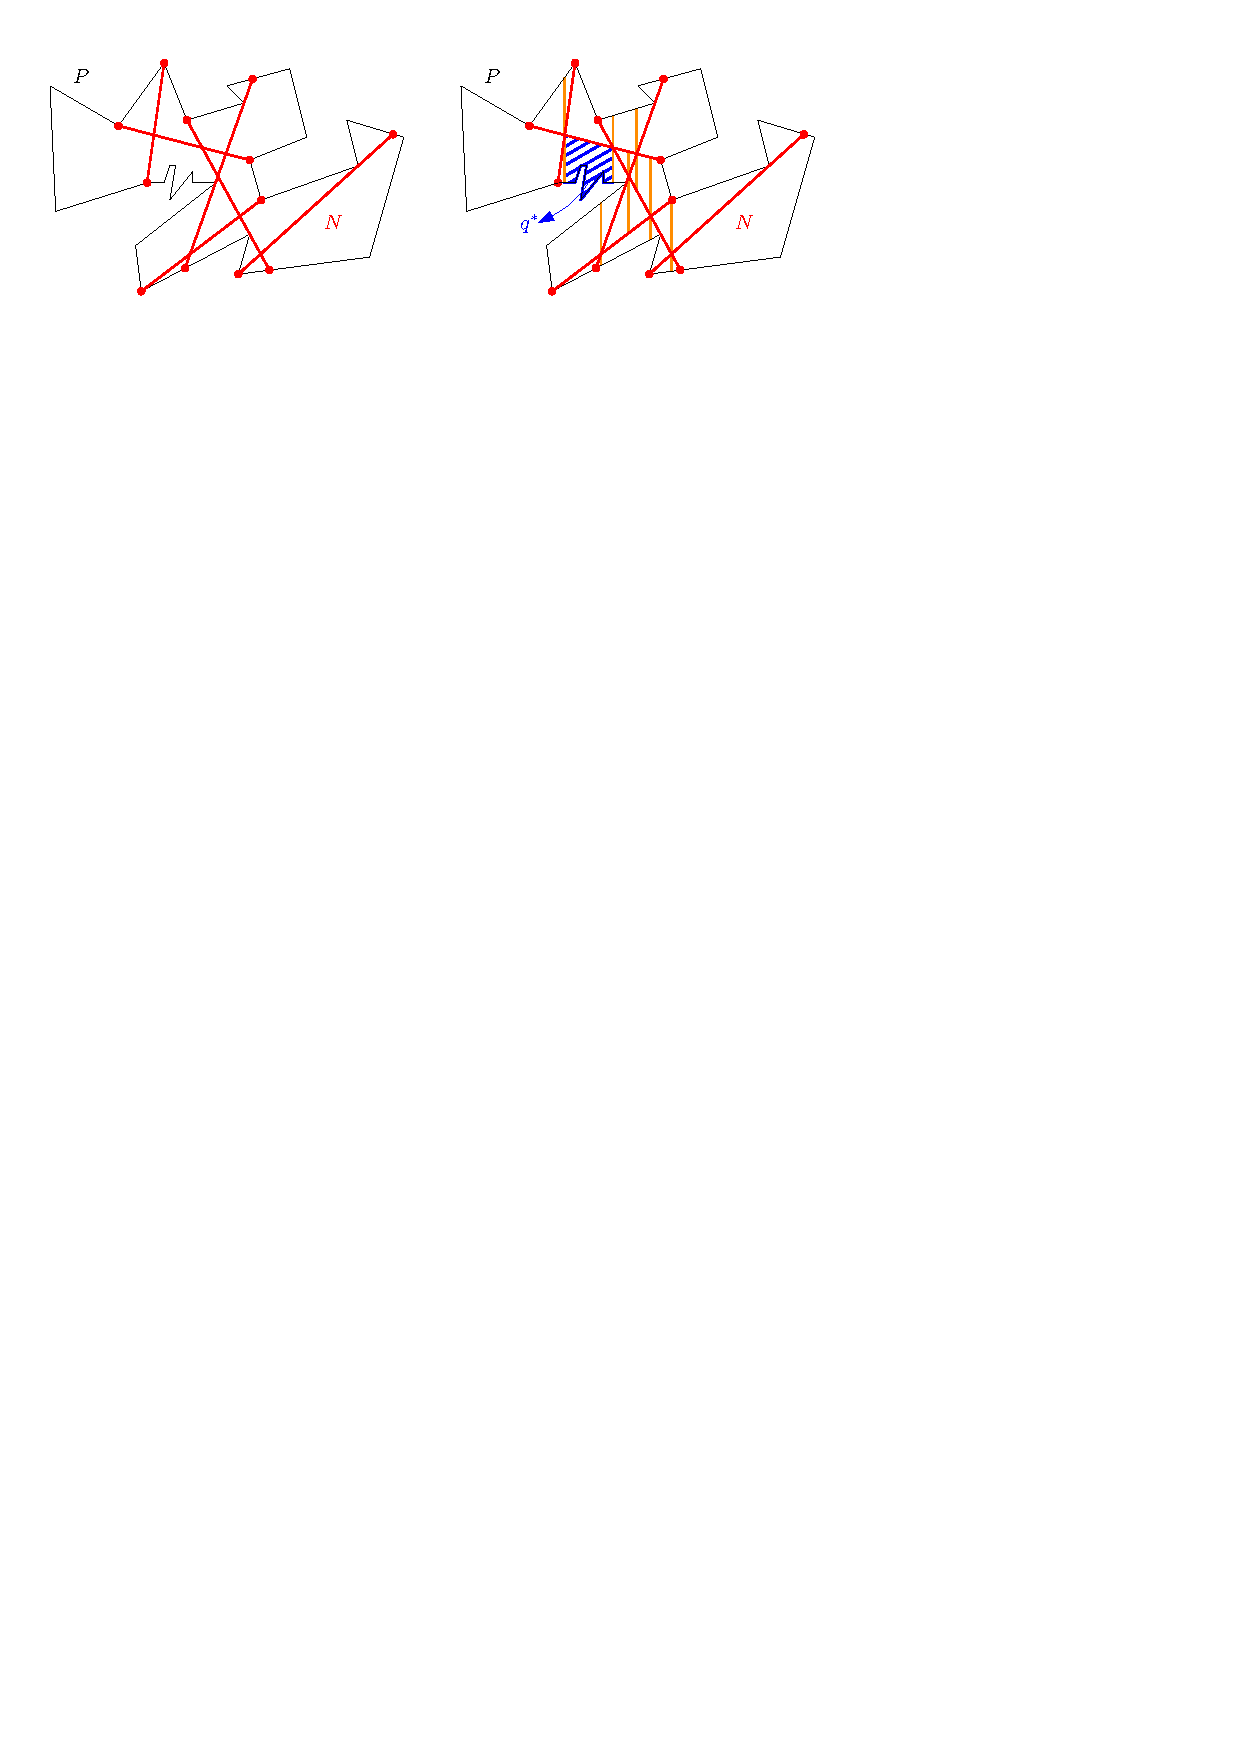
\includegraphics{img/CuttingOfChords.pdf}

\caption{\small }
\label{fig:Cutting of Chords}
\end{figure}

We want to decide now which $R$-trapezoid contains the geodesic center of $P$. 
To this end, for each edge of an $R$-trapezoid, we can extend it to a chord $C$ by doing two ray-shooting queries in $O(m)$ time. Then, we can use the second part of the relative center algorithm introduced by Pollack et al.~\cite[Section~3]{pollackComputingCenter} to find the point on $C$ that minimizes $\F{P}{x}$ (during the first part of their algorithm they compute the equivalent of apex functions restricted to $C$).
This algorithm is an extension of the linear programming technique introduced by Megiddo~~\cite{megiddo1982linear}. 
The only requirement of this technique is that the function $\F{P}{x}$ coincides with the upper envelope of the apex functions when restricted to $C$.

Recall that $\tau_R$ consists of all the apexed triangles that intersect $R$. 
Thus, we have all the apexed triangles that intersect $C$. Consequently, Lemmas~\ref{lemma:Triangles inside hourglasses} and~\ref{lemma:Triangles inside funnels} imply that the upper envelope of the apex functions coincides with $\F{P}{x}$ when restricted to $C$.
Let $p\in C$ be the point that archives the minimum of $\F{P}{x}$ (note that $p$ may be an endpoint of $C$). 
We want to decide now on which side of $C$ lies the optimum of $\F{P}{x}$, i.e., the geodesic center of $x$. 
To this end, we consider the apexed triangles whose apex functions define the value of $\F{P}{x}$ at~$p$. 
They can be found in $O(m)$ time by looking at all the apexed triangles of $\tau_R$ that contain~$p$. 
We then consider the definers of these apexed triangles. By looking at their distance function to $p$, which is encoded by the apex functions, we can decide locally on which side of $C$ the function decreases and determine the side that contains the optimum of $\F{P}{x}$.

Because the algorithm described by Pollack et al.~\cite[Section~3]{pollackComputingCenter} runs in linear time on the number of functions defined on $C$, we can decide in total $O(m)$ time on which side of $C$ the geodesic center of $P$ lies. 

Because our decomposition into $R$-trapezoids has constant complexity, we need to perform this test only $O(1)$ times before determining the $R$-trapezoid $q^*$ that contains the geodesic center of $P$. 
Since $N$ is a $\varepsilon$-net, we know that at most $\varepsilon |C|$ chords of $C$ intersect $q^*$.

If $q^*$ is contained in the interior of $R$, then $q^*$ is convex. In this case, we have found a convex trapezoid that contains the solution and this algorithms finishes. Otherwise, $q^*$ is a $P$-cell bounded by at most three segments, say $\alpha, \beta$ and $\gamma$, and some $P$-chain $R_{q^*}$; see Figure~\ref{fig:Cutting of Chords}. 
In order to proceed with the algorithm on  $q^*$ recursively, we need to compute the set $\tau_{q*}$ of at most $\varepsilon |C|$ apexed triangles of $\tau_R$ that intersect $q^*$. We proceed as follows.

For each apexed triangle $\triangle\in \tau_R$, we consider the index of its endpoints and test in $O(1)$ time if any of them lies on the $P$-chain $R_{q^*}$. If they do, then they intersect $q^*$. Otherwise, we know that this triangle has no endpoint in $R_{q^*}$ and could only intersect $q^*$ if one of its edges intersects either $\alpha, \beta$ or $\gamma$. Since this can be tested in $O(1)$ time, we conclude that the at most $\varepsilon |C|$ triangles of $\tau_R$ that intersect $q^*$ can be found in $O(m)$ time.
Because $|C| \leq 2m$, we guarantee that at most $2\varepsilon m$ apexed triangles intersect $q^*$. 
Moreover, because each vertex of $q^*$ is in at least one apexed triangle of $\tau_R$ and from the fact that each apexed triangle covers at most three vertices, we conclude that $q^*$ consists of at most $6 \varepsilon m$.
Thus, by choosing $\varepsilon = 1/12$, we guarantee that both the size of the $P$-cell $q^*$ and the number of apexed triangles in $\tau_{q^*}$ are at most $m/2$.

By recursing on $q^*$, we guarantee that after $O(\log m)$ iterations, we will find either a convex trapezoid contained in $R$ that contains the center, or we reduce the size of $\tau_R$ to a constant in which case the optimum of $\F{P}{x}$ can be found using an exhaustive search in $O(1)$ time. Since we halve the the size of the $P$-cell and the number of apexed triangles in each iteration, the total running time of this algorithm is given by the recurrence $T(m) = T(m/2) + O(m)$ which solves to $T(m) = O(m)$. 
Because $|\tau| = O(n)$ by Lemma~\ref{lemma:Size of tau}, the total running time of this algorithm on $P$ is $O(n)$.

\begin{lemma}\label{lemma:Finding the convex trapezoid}
In $O(n)$ time we can find either the geodesic center of $P$ or a convex trapezoid containing this geodesic center.
\end{lemma}


\section{Solving the problem restricted to a convex trapezoid}\label{Section:Solving convex optimization poblem}
In the previous section we show how to find either the geodesic center of $P$, or a convex trapezoid $q^*$contained in $P$ that contains this center. 
Recall that $\phi(x)$ denotes the upper envelope of the apex functions of every triangle in $\tau$.
The important thing to notice is that, as in the case of chords, the function $\phi(x)$ restricted to $q^*$ is a convex function, which allows us to do prune and search using cuttings.

Let $\triangle_{1}, \triangle_{2}, \ldots, \triangle_{m}$ be the set of $m= O(n)$ apexed triangles of $\tau$ that intersect $q^*$. Let $g_i(x) = |x a_i| + \kappa_i$ be the apex function of $\triangle_i$, where $a_i$ and $w_i$ are the apex and the definer of $\triangle_i$, respectively, and $\kappa_i = \g{a_i, w_i}$ is a constant.

Recall that the geodesic center of $P$ is the point in $P$ that minimizes the function $\F{P}{x}$.
By Lemma~\ref{lemma:Optimization problem same as geodesic center}, $\phi(x) = \F{P}{x}$. 
Therefore, the problem of finding the point that minimizes $\F{P}{x}$ can be reduced to the following optimization problem in $\mathbb{R}^3$:

\textbf{(P1).} Find a point $(x,r)\in \mathbb{R}^3$ minimizing $r$ subject to $x\in q^*$ and
$$\text{$g_i(x) = |x a_i| + \kappa_i \leq r$, if $x\in \triangle_{i}$ for $1\leq i \leq m$}.$$

Thus, we need only to find the solution to (P1) to find the geodesic center of $P$.
A similar optimization was studied by Megiddo in~\cite{megiddo1989ball}. 
The main difference being that we have apex functions, defined only in their corresponding apexed triangles, instead of functions defined in the entire plane. 

We use some remarks described by Megiddo in order to simplify the description of (P1).
To simplify the formulas, we square the equations:
$$g_i(x) = \|x\|^2 + 2x\cdot a_i + \|a_i\|^2  = |x a_i|^2 \leq (r - \kappa_i)^2 = r^2 - 2r\kappa_i + \kappa_i^2$$ 
And finally for each $1\leq i\leq m$, we define the function $h_i(x, r)$ as follows:
$$h_i(x, r) = \|x\|^2 + 2x\cdot a_i + \|a_i\|^2  - r^2 + 2r\kappa_i - \kappa_i^2 \leq 0$$

Therefore, our optimization problem can be reformulated as:

\textbf{(P2).} Find a point $(x,r)\in \mathbb{R}^3$ such that $r$ is minimized subject to $x\in q^*$ and 
$$h_i(x, r) \leq 0, \text{ if $x\in \triangle_{i}$ for $1\leq i \leq m$}.$$%\text{ and } r > \max\{\kappa_i\}

Although the functions $h_i(x,r)$ are not linear, they all have the same non-linear terms. Therefore, for $i\neq j$, we get that
$h_i(x,r) = h_j(x, r)$ defines a \emph{separating plane}
$$\gamma_{i,j} = \{(x, r) \in \mathbb{R}^3: 2 (a_i - a_j) \cdot x - 2( \kappa_i - \kappa_j) r = \|a_i\|^2 - \|a_j\|^2 - \kappa_i^2 + \kappa_j^2\}$$

As noted by Meggido, this separating plane has the following property:
If the solution $(x, r)$ to our optimization problem is known to lie to one side of $\gamma_{i,j}$, then we know that one of the constraints is redundant. 

In Megiddo's problem, it sufficed to have a \emph{side-decision algorithm} to determine on which side of a plane $\gamma_{i,j}$ the solution lies. Megiddo showed how to implement such an algorithm in linear time on the number of constraints~\cite{megiddo1989ball}.

Using this side-decision algorithm, he shows how to solve the optimization problem. A variant of his technique could be described as follows: Start by pairing the functions arbitrarily, and then consider the set of separating planes defined by these pairs.
For some constant $r$, compute a $1/r$-cutting in $\mathbb{R}^3$ of the separating planes.
An $1/r$-cutting is a partition of the plane into $O(r^2)$ convex cells of constant size such that each intersects at most $n/r$ separating planes.
A cutting of planes can be computed in $O(n)$ time in $\mathbb{R}^3$ for any $r = O(1)$~\cite{matousekCuttings}.
After computing the cutting, determine in which of the cells the optimum lies by performing $O(1)$ calls to the side-decision algorithm. 
Because at least $(r-1)n/r$ separating planes do not intersect this constant size cell, for each of them we can discard one of the constraints as it becomes redundant. Repeating this algorithm recursively we obtain a linear running time.

In this paper, we follow a similar approach, but our set of separating planes needs to be extended in order to handle apex functions as they are only partially defined.
Note that each apexed triangle that intersects $q^*$ has its endpoints either outside of $q^*$ or on its boundary, i.e., each chord bounding an apexed triangle splits $q^*$ into two convex regions.

\subsection{Optimization problem in a convex domain}
In this section we describe our algorithm to solve the optimization problem (P2). 
%\textbf{(P2).} Find a point $(x,r)\in \mathbb{R}^3$ such that $r$ is minimized subject to $x\in q^*$ and 
%$$h_i(x, r) \leq 0 \text{ and } r > \max\{\kappa_i\}\ (1\leq i\leq m), \text{if $x\in \triangle_{i}$ for $1\leq i \leq m$}.$$
To this end, we start by pairing the apexed triangles arbitrarily to obtain $m/2$ pairs.
By identifying the plane where $P$ lies with the plane $Z_0 = \{(x,y,z): z = 0\}$, we can embed each apexed triangle in $\mathbb{R}^3$.
A \emph{plane-set} is a set consisting of at most five planes in $\mathbb{R}^3$.
For each pair $(\triangle_i, \triangle_j)$ we define a plane-set as follows: 
For each chord bounding either $\triangle_i$ or $\triangle_j$, consider the line extending this chord and the vertical extrusion of this line in $\mathbb{R}^3$, i.e.,  the plane containing this chord orthogonal to $Z_0$. Moreover, consider the separating plane~$\gamma_{i,j}$. The set containing these planes is the plane-set of the pair $(\triangle_i, \triangle_j)$.

Let $\Gamma$ be the union of all the plane-sets defined by the $m/2$ pairs of apexed triangles. Thus, $\Gamma$ is a set that consists of $O(m)$ planes. Compute an $1/r$-cutting of $\Gamma$ in $O(m)$ time for some constant $r$ to be specified later.
Because $r$ is constant, this $1/r$-cutting splits the space into $O(1)$ convex cells, each bounded by a constant number of planes~\cite{matousekCuttings}. 
By using a side-decision algorithm (to be specified later), we can determine the cell $Q$ of the cutting that contains the solution. Because $Q$ is the cell of a $1/r$-cutting of $\Gamma$, we know that at most $|\Gamma|/r$ planes of $\Gamma$ intersect $Q$. In particular, at most $|\Gamma|/r$ plane-sets intersect $Q$ and hence, at least $(r-1)|\Gamma|/r$ plane-sets do not intersect $Q$. 

Let $(\triangle_i, \triangle_j)$ be a pair such that its plane-set does not intersect $Q$. 
Let $Q'$ be the projection of $Q$ on the plane $Z_0$. Because the plane-set of this pair does not intersect $Q$, we know that $Q'$ intersects neither the boundary of $\triangle_i$ nor that of $\triangle_j$.
Two cases arise:

\textbf{Case 1.} If either $\triangle_i$ or $\triangle_j$ does not intersect $Q'$, then we know that their apex function is redundant and we can drop the constraint associated with this apexed triangle.

\textbf{Case 2.} If $Q'\subset \triangle_i\cap \triangle_j$, then we need to decide which constrain to drop. 
To this end, we consider the separating plane $\gamma_{i,j}$. Notice that inside the vertical extrusion of $\triangle_i\cap \triangle_j$ (and hence in $Q$), the plane $\gamma_{i,j}$ has the property that if we know its side containing the solution, then one of the constraints can be dropped. Since $\gamma_{i,j}$ does not intersect $Q$ as $\gamma_{i,j}$ belongs to the plane-set of $(\triangle_i, \triangle_j)$, we can decide which side of $\gamma_{i,j}$ contains the optimum and drop one of the constraints.
\vspace{.05in}

Regardless of the case if the plane-set of a pair $(\triangle_i, \triangle_j)$ does not intersect $Q$, then we can drop one of its constraints. Since at least $(r-1)|\Gamma|/r$ plane-sets do not intersect $Q$, we can drop at least $(r-1)|\Gamma|/r$ constraints.
Because $|\Gamma| \geq m/2$ as each plane-set contains at least one plane, by choosing $r = 2$, we are able to drop at least $|\Gamma|/2 \geq m/4$ constraints.
Consequently, after $O(m)$ time, we are able to drop $m/4$ apexed triangles.
By repeating this process recursively, we end up with a constant size problem in which we can compute the upper envelope of the functions explicitly and find the minimum using exhaustive search. 
Thus, the running time of this algorithm is bounded by the recurrence $T(m) = T(3m/4) + O(m)$ which solves to $O(m)$. 
Because $m = O(n)$, we can find the solution to (P2) in $O(n)$ time.

The last detail is the implementation of the side-decision algorithm. 
Given a plane $\gamma$, we want to decide on which side lies the optimum of (P2).
To this end, we solve (P2) restricted to~$\gamma$, i.e., with the additional constraint of $(x,r)\in \gamma$. 
This approach was used by Megiddo~\cite{megiddo1989ball}, the idea is to recurse by reducing the dimension of the problem.
Another approach is to find this using the algorithm described by Pollack et al.~\cite[Section~3]{pollackComputingCenter}. 

Once the optimum of (P2) restricted to $\gamma$ is known, we can follow the same approach used by Megiddo~\cite{megiddo1989ball} to find the side of $\gamma$ containing the global optimum. 
Intuitively, we find the apex functions that define the optimum restricted to $\gamma$. Since $\phi(x) = \F{P}{x}$ is locally defined by this functions, we can decide on which side the optimum lie using convexity.
We obtain the following result.

\begin{theorem}
Let $q^*$ be a convex trapezoid contained in $P$ such that $q^*$ contains the geodesic center of $P$. Given the set of all apexed triangles of $\tau$ that intersect $q^*$, we can compute the geodesic center of $P$ in $O(n)$ time.
\end{theorem}

\begin{corollary}
Given a simple polygon $P$ with $n$ vertices, we can compute its geodesic center in $O(n)$ time.
\end{corollary}

\section{Conclusions}

\bibliographystyle{abbrv}
\bibliography{Geodesic}


\end{document}
